\chapter{Resonance Searching Strategy}
\chapterquote{The wilderness must be explored!}{Russell, Up}
The resonance search is applying a general strategy with three benchmarks for the exotic particles of different spins: the narrow width approximated scalar boson (NWA, spin=0), the heavy vector triplet (HVT W', Z' bosons, spin=1), and the Randall-Sundrum graviton (RSG, spin=2).
In the study in this thesis, $WW$ and $WZ$ are the two medium states of interest through the production of gluon-gluon fusion, Drell-Yan process, or vector boson fusion. The vector boson fusion is the fusion process of two vector bosons ($W$ or $Z$) emitted from two incoming quarks, and the two quarks are then scattered into two energetic jets with wide $\eta$ separation and high invariant mass. The production processes could be seen in Fig. \ref{Fig:Xprod} as Feynman diagrams. The strategy herein considers only final states in which one $W$ boson decays leptonically ($W\rightarrow l\nu$) into an electron or muon accompanied by a neutrino of the corresponding flavour, while the other $W$ or $Z$ boson is chosen to decay hadronically into two quarks reconstructed into two $R=0.4$ jets or one $R=1.0$ jet ($W/Z\rightarrow jj$ or $W/Z\rightarrow J$). The tau decay channel is not considered in thsi analysis. The benefit of choosing this final state is to have the high branch ratio from the hadronic decay and suppress the QCD contamination by the leptonic side. This study is conducted in a wide range of candidate particle mass ranging from $300GeV$ to $5TeV$. If the mass of a resonance particle is high enough ($m>\tilde1~TeV$), the outcoming two quarks in the final state would be highly boosted, so they cannot not be resolved as two jets with $R=0.4$, and a larger cone of $R=1.0$ is applied to collect their signatures into a single fat jet. 
\\
\\This search was performed with the $36.1fb^{-1}$ data collected by the ATLAS detector in 2015 and 2016 with pp collisions at $\sqrt{s}=13~TeV$. 

\begin{figure}[htp]
	\centering
	\subfloat[Drell-Yan Process]{\includegraphics[width=.3\textwidth]{Chapter3/DY_X.pdf}}\hfill
	\subfloat[gluon-gluon Fusion]{\includegraphics[width=.3\textwidth]{Chapter3/ggF_X.pdf}}\hfill
	\subfloat[Vector Boson Fusion]{\includegraphics[width=.3\textwidth]{Chapter3/VBF_X.pdf}}
	\caption{The Feynman diagrams of different production mechanisms for particle X which decays into two SM bosons.}
	\label{Fig:Xprod}
\end{figure}
\section{Signal Models}
\label{sec:signal_intro}
In the SM, bosons are the force carriers and also maintain the conservation of certain physical quantities associated with underlying symmetries. To seek for the solution of unsolved problems of the SM, many new models predict the existence of new bosons corresponding to unknown interactions or symmetries, and they also have the strong coupling to the SM bosons which provide the access to verify those theories. However, the existing new models are constructed with many free parameters, and each set of them needs a dedicated analysis from the experimental side, which is impossible in reality. Therefore, a simplified model with only the kinematic parameters related to resonance mass is introduced for which experiments provide precise measurements for on-shell bosons.  
\\
\\This strategy could scan through many models, so it is defined as a general search. However, to give a better separation between signal and background, three benchmarks are applied in this analysis for sensitivity optimization which corresponds to bosons with different spins: $spin=0$, narrow width approximation Higgs bosons (NWA); $spin=1$ heavy vector triplets (HVT); $spin=2$, Randall–Sundrum model gravitons (RSG).
\\
\\{\bf Narrow Width Approximation Higgs Boson}
\\
Some extended models predict the existence of high mass Higgs bosons to solve the problems with the Higgs boson naturalness. However, as only kinematic properties are concerned, the interpretation model chosen in this analysis is the SM Higgs boson but with higher mass. To have further simplification, the decay of the Higgs boson is forced to be always at the mass pole with the narrow width approximation. This means the transferred momentum, $q$, from the proton partons is exactly the mass of the resonant particle under the assumption, which gives the narrow resonance width, $\Gamma/m_{H}<<1$, and the interference to the SM Higgs boson is taken negligible\cite{NWAInterference}. Therefore, the Relativistic Breit–Wigner distribution could be written as:
\begin{equation}
f(q) = \frac{k\pi}{M\Gamma}\delta(q^2-m_{H}^2)
\end{equation}
where $k$ represents:
\begin{equation}
k=\frac{2\sqrt{2}m_{H}\Gamma\gamma}{\pi\sqrt{m_{H}^2+\gamma}}
\end{equation}
and $\gamma=\sqrt{m_{H}^2(m_{H}^2+\Gamma^2)}$. This is then used to evaluate the cross-section of the Higgs boson production.
\\
\\{\bf Heavy Vector Triplet}
\\
\\Heavy vector bosons are predicted by many new BSM theories with the coupling to quarks, leptons, SM vector bosons and Higgs bosons, which constructs a wide phase space to explore. To examine the suitable theories, this study attempts to investigate all the couplings with the set-up of one neutral heavy boson, $Z'$, and two degenerate charged bosons, $W'^{\pm}$, with the given coupling constant, $g_{V}$. For optimization,  two models are taken as the benchmarks\cite{Pappadopulo:2014qza,deBlas:2012qp}. Model A is with an additional symmetry breaking to SM, $SU_{1}(2)\times SU_{2}(2) \times U(1) \rightarrow SU_{L}(2) \times U(1)$ giving a weak coupling: $g_{V} \sim \mathcal{O}(1)$. For the scenario of a strong SM boson coupling, the Minimal Composite Higgs Model is taken as model B with the symmetry breaking, $SO(5) \rightarrow SO(4)$ for $4\pi \geq g_{V} \geq 1$. However, because the decay width is proportional to the coupling constant, and the focus of this search is for the narrow resonance, only $6 \geq g_{V} \geq 1$ is considered with $\Gamma_{V'}/m_{V'}$ below $10\%$.
\\
\\To simplify the models, the coupling strength to all fermions are equal with the scale of $g^2c_{F}/g_{V}$ where $g$ is the $SU_{L}(2)$ gauge coupling, and $c_{F}$ is the dimensionless coefficient between bosons and fermions defined as a free parameters of order one in the phase space of interest. As the fermionic coupling scale is proportional to $1/g_{V}$, model A turns to be more sensitive to the fermionic production with Drell-Yan process, while it is suppressed in model B. In contrast, the coupling to bosons is governed by $c_{H}g_{V}$ with $c_{H}$ as the universal coupling among bosons. Therefore, model B has better sensitivity for higher branch ratio of the decay channel of diboson in this analysis than model A. For the interpretation, the two parameters, $g^2c_{F}/g_{V}$ as well as $c_{H}g_{V}$, construct a two-dimension phase space across which production rates and decay branching ratios vary significantly. 
\\
\\As the coupling to all bosons are the same ($c_{H}g_{V}$), the neutral and charged heavy boson ($Z'$ and $W'^{\pm}$) have the same decay branch ratio to all SM bosons:
\begin{equation}
BR(Z'\rightarrow ZH) = BR(Z'\rightarrow W^\pm W^\pm) = BR(W'^\pm \rightarrow W^\pm Z) = BR(W'^\pm \rightarrow W^\pm H)
\end{equation}
However, with the small mixing angle (between SM and BSM bosons), the coupling in the transverse component is well suppressed, and the dominant contribution is from the longitudinal component. For the same reason, the couplings to neutral dibosons and $W\gamma$ are also so weak that those channels are ignored in this analysis. In the other case, the coupling to $HH$ is forbidden due to the concern of momentum and angular momentum conservation. 
\\
\\{\bf Randall-Sundrum Graviton}
\\
\\To solve the hierarchy problem, extra dimensions were proposed as one of the solutions\cite{Randall:1999ee}. It leads to the result that the effective Planck scale, $M_{pl}=2\times10^{18}GeV$, is determined by the existence of extra dimensions from the orginal scale, $M$, and the extra-dimension geometry. The relation between $M_{pl}$ and $M$ is: 
\begin{equation}
\label{Eq:planck_relation}
M_{pl}^{2} = M^{n+2}V_{n}
\end{equation}
where n is the number of dimensions which are not yet observed, and $V$ is the volume constructed from the extra dimensions regardless of the four-dimensional spacetime. Therefore, the visible spacetime is just a manifold under ($4+n$) dimensions.
\\ 
\\Under Randall-Sundrum model, only one more dimension is needed, which hypothesizes that the fifth dimension is constrained with boundary condition of the $\phi$ periodicity ranged between $-\pi$ to $\pi$ called the ``warped bulk'' which bridges two four-dimensional manifolds at $\phi=\pi$  and $\phi=0$ ($\phi$ is taken as the fifth coordinate). The ``Hilbert-Einstein''action under the set-up could be presented as:
\begin{equation}
S = S_{gravity} +S_{obs} + S_{hid}
\end{equation}
\begin{equation}
S_{gravity} = \int d^4x \int^{\pi}_{-\phi}d\phi\sqrt{G}\left[-\Lambda +2M^3R\right]
\end{equation}
\begin{equation}
S_{vis(hid)} = \int d^4x\sqrt{-g_{vis(hid)}}\left[\mathcal{L}_{vis(hid)}-V_{vis(hid)}\right]
\end{equation}
with $\Lambda$ as the cosmological constant, R as the scalar spacetime curvature, and $g$'s are the determinants of metric tensor matrix,  $g_{\mu\nu}$, $V_{vis}$, and $V_{hid}$ are the constant gravitational potentials taken out from the Lagrangian vacuum energy for the visible and hidden spacetimes. After inserting the terms into the Einstein Feild Equation, it leads to the solution for the spacetime description:
\begin{equation}
ds^2=e^{-2\sigma(\phi)}\eta_{\mu\nu}dx^\mu dx^\nu + r_c^2 d\phi^2
\end{equation}
with
\begin{equation}
\sigma(\phi) = kr_c|\phi| \quad k=\sqrt{\frac{-\Lambda}{24M^3}}
\end{equation}
where $\eta$ is the Minkowski metric, and $r_{c}$ is the constant independent of $\phi$ taken as the ``compactification radius'' of the extra dimension on the orbifolding. As a result, the extra dimension only has the dimensional interval, $\pi r_{c}$, at $\phi=\pi$ in the visible spacetime. Taking the space description into Eq. \ref{Eq:planck_relation}, the relation between $r_c$ and $M_{pl}$ could be derived as:
\begin{equation}
M_{pl}^2=\frac{M^3}{k}\left[1-e^{-2kr_{c}\pi}\right]
\end{equation}
This expression indicates that $M_{pl}$ depends on $kr_{c}$, and the weak gravity could be explained with a proper choice of $r_c$. Under the solution, the existence of graviton (the gravitational field) is then taken as the tensor fluctuation on Minkoski metric: $\eta_{\mu\nu} \rightarrow \eta_{\mu\nu}+\bar{h}_{\mu\nu}(x)$. To estimate its mass, the new spacetime geometry is inserted into the Higgs sector in the SM Lagrangian, and it gives the result: $m=e^{-kr_{c}\pi}m_{0}$ with $m_{0}$ as the original mass scale in the visible manifold (IR brane), and m as the one in the five-dimensional spacetime. (This relation could also be applied to SM particles.) If $e^{kr_{c}\pi}$ is of the order $10^{15}$, the mass scale would be in the scale of $TeV$ under the mechanism which offers the signature verifiable to the LHC energy scale with the couplings to SM particles derived from the same way.
\section{Simulation Samples and Derivation}
Each SM background process and each signal sample are simulated by the procedure mentioned in \ref{sec:simulation}.  To make a proper comparison between the simulation and data, the event numbers are normalised to the theoretical cross section and total data luminosity. However, the modelling of interactions between the ATLAS detector and particles is not perfect, and it leads to the discrepancy in efficiency measurements including the particle reconstruction, lepton isolation, trigger, and jet b-tagging efficiency. To recover this disagreement, scaling factors are estimated from the comparison between data and MC and applied on the event weight in the MC samples. 
\\
\\Another disagreement comes from the inconsistency in distribution of interaction number per bunching crossing , $\mu$. To eliminate the effect, one more scale factor is applied through the process called ``pile-up reweighting'' (PRW) to make the simulated $\mu$ distribution agree with data. 
\\
\\After considering all the factors for the data-MC comparison, the final simulation event yield could be reweighted to data by:
\begin{equation}
N_{yield} = \mathcal{L}\times XS \times \epsilon_{rec} \times \epsilon_{iso} \times \epsilon_{trigger} \times \epsilon_{b-tagging} \times \epsilon_{prw} / N_{mc}
\end{equation}
where $N_{mc}$ is the total event weight from simulation, and $\epsilon$'s stand for the scaling factors of different contributions. 
\\
\\{\bf Background Simulation}
\\
\\Some of the SM processes have the same final state to the new physics of our interest: one lepton, one neutrino and multiple jets, and they are called ``irreducible'' background which could not be well-suppressed by selection cuts. This type of backgrounds are estimated from the Monte Carlo simulation contributed from W+jets ($W\rightarrow l\nu$), $t\bar{t}$ ($t\rightarrow bW \rightarrow bjj$ and $t\rightarrow bW \rightarrow bl\nu$), diboson ($WW/WZ\rightarrow l\nu jj$), Z+jets ($Z\rightarrow ll$), and single top interactions.  
\\
\\The events of W/Z+jets are simulated by \textsc{SHERPA} v2.2.1\cite{sherpa22_twiki}, with the PDF configuration of \textsc{NNPDF30NNLO}\cite{Ball:2012cx} as the baseline generator, and the simulation uncertainty is taken by the comparison to other generators detailed in next chapter. With the complicated process of hadronisation including the broad range of jet $p_{T}$ and involved quark flavours, the simulation is done respectively with multiple slices of $max(h_{T}, p_{T}(W/Z))$ ($h_{T}$ is the scalar sum of $p_{T}$ from all jets) and different number of bottom and charm quarks. The involved matrix element for the simulation are up to 2 partons at NLO and 4 partons at LO which is followed by merging into the Sherpa parton shower. The resulting cross section for normalisation is estimated to NNLO of QCD.
\\
\\$t\bar{t}$ events are generated through \textsc{Powheg-Box}\cite{Alioli:2010xd} v2 with the matrix element calculation provided by \textsc{CT10 PDF}\cite{Gao:2013xoa} with the top quark mass set at $172.5GeV$, and the \textsc{HDAMP} parameters for high $p_{T}$ radiation is set at $1.5m_{t}$. Different from \textsc{SHERPA} as a self-contained generator to do parton shower itself, the simulation from \textsc{Powheg-Box} is then interfaced through \textsc{MadSpin}\cite{Artoisenet:2012st} and \textsc{PYTHIA}8.186 tuned by Perugia 2012 (P2012)\cite{mc11ctunes} and \textsc{CTEQ6L1 PDF}\cite{Stump:2003yu} sets for spin correlation preservation of top quark decays and the following parton shower, fragmentation and underlying events. The renormalisation and factorisation scale of the whole process are determined by $\sqrt{m_{t}^2+p^2_{T}(t)}$. The $t\bar{t}$ cross section used for normalisation is calculated using \textsc{TOP++} 2.0\cite{Czakon:2013goa} with the precision up to NNLO in QCD. To take in the contribution from soft gluon terms, a re-summation with next-to-next-to-leading logarithmic (NNLL) is applied to make further correction.  
\\
\\Single top events are generated through three processes: s-, t- and Wt-channel productions (Feynman diagrams are presented in Fig. \ref{Fig:singletop}). For the simulation of Wt and s-channels, the same recipe from $t\bar{t}$ generation is adopted, while the t-channel one is through \textsc{Powheg-Box} v1 with fixed four-flavor \textsc{CT10f4 PDF}\cite{Lai:2010vv} set but also followed by the same procedure for decay and parton showering from $t\bar{t}$ generation. The renormalisation and factorisation scales are set respectively for the three channels with:
\begin{itemize}
	\item s-channel $\&$ Wt-channel: $m_{t}$
	\item t-channel 4\times$\sqrt{m_{q}^2+p^2_{T}(q)}$ (q is the quark  associated with the single top quark production)
\end{itemize}
, and the cross section for each production is calculated separately with the description in \cite{Kidonakis:2011wy,Kidonakis:2010ux}
\begin{figure}[htp]
	\centering
	\subfloat[t-channel]{\includegraphics[width=.25\textwidth]{Chapter3/t-channel.png}}\hfill
	\subfloat[Wt-channel]{\includegraphics[width=.3\textwidth]{Chapter3/Wt-channel.png}}\hfill
	\subfloat[s-channel]{\includegraphics[width=.3\textwidth]{Chapter3/s-channel.png}}
	\caption{The Feynman diagrams of three channels for single top production.}
	\label{Fig:singletop}
\end{figure}

The generation of $WW/WZ$ events are also through \textsc{SHERPA} v2.2.1 for the event production and the hadronisation. 
\\
\\{\bf Signal Simulation}
\\
\\HVT samples are generated via \textsc{MADGRAPH5}\cite{Alwall:2014hca} interfaced to \textsc{PYTHIA8}\cite{Sjostrand:2007gs} with the the resonance mass points ranged from $300~GeV$ to $5~TeV$ of $100~GeV$ spacing. For simplicity, $g_V=1$ and $g_V=3$ are set for model A and model B respectively.
\\
\\RS graviton events are also simulated through \textsc{MADGRAPH5} and \textsc{PYTHIA8}, and only the ggF production is considered for this signal. Within the simulation, $r_{c}=1$ is set as the default for the simulation, but it is also reweighted in the resonance mass distribution at parton level for $r_{c}=0.5$. This is for the comparison with the result from the CMS collaboration. The decay width of this configuration is expected to be $\approx6\%$. 
\\
\\The decay width and cross section of HVT and RS graviton are summarised in tab.~\ref{Tab:xs_decaywidth}. For the NWA Higgs boson, its interference to the SM Higgs boson ($125~GeV$) is assumed to be negligible as discussed in \ref{sec:signal_intro}. Its narrow decay width is set as a constant at $4.07~MeV$ for all mass points which is beyond the experimental resolution with the production of ggF and VBF, which are simulated separately. The simulation is done by \textsc{Powheg-Box} v2 showered with \textsc{PYTHIA8} under \textsc{CTEQ6L1} PDF set. 
\begin{table}[htb]
	\caption{The decay width and cross section of HVT and RSG at $800GeV$, $1.6TeV$, and $2.4TeV$ mass points}
	\centering
		\begin{tabular}{|c|ccc|cc|}
          \hline
          \hline
                   & \multicolumn{3}{c|}{ HVT W' and Z' }                                     & \multicolumn{2}{c|}{ RS $G*$}  \\
              $m$  & $\Gamma$ & $\sigma \times BR(Z' \to WW)$ & $\sigma \times BR(W' \to WZ)$ & $\Gamma$ & $\sigma \times BR(G* \to WW)$ \\
            $[TeV]$& $[GeV]$  & $[fb]$                        & $[fb]$                        & $[GeV]$  & $[fb]$      \\
          \hline
               0.8 & 32       & 354                           & 682                           & 46       & 301   \\
               1.6 & 51       & 38.5                          & 79.3                          & 96       & 4.4 \\
               2.4 & 74       & 4.87                          & 10.6                          & 148      & 0.28 \\
          \hline
         \end{tabular}
	\label{Tab:xs_decaywidth}
\end{table}
\noindent
\\
\\{\bf Derivation}
\\
\\For practical reasons , the analyses were not run on AODs directly. Instead, they went through the ``derivation'' procedure composed of ``trimming'' and ``slimming'' to drop down variables and events of no interest first\cite{Borodin:2015wqa}, which outputs the data format called derived AOD (DAOD). For the broad variety of analysis types, a couple of derivation schemes are applied, and the analyese with similar final states share the same derivation scheme. 
\\
\\With the final state of this analysis, ``HIGG5D2'' is chosen with the derivation scheme as the following:
\begin{itemize}
  \item trigger: passing at least one electron, muon, or $E^{T}_{missing}$ trigger
  \item lepton: one electron or muon with $p_{T}>15~GeV$ 
  \item jet: two small R jets with $p_{T}>20~GeV$, one  small R jet with $p_{T}>100~GeV$, or one large R jet with $p_{T}>150~GeV$
\end{itemize}
\section{Physical Object Definition}
Because the LHC is using protons as the beam source, it leads to the enormous production of hadronic jets. Within the environment, most reconstructed objects have the potential to suffer from great contamination from jet misidentified as other objects. Therefore, the object definitionn for this anlysis is to keep the signal efficiency and significant suppression of misidentification of the intended objects at the same time. 
\\
\\{\bf Electron}
\\
\\The electrons in this analysis are defined as two types, loose and signal, and each event only has exactly one signal lepton without additional loose one. Signal electrons are required to have $p_{T}$ above $27~GeV$ to reach the trigger efficiency turn-on plateau, and $|\eta|<2.47$ is applied on both electron types within the acceptance of inner detector with the crate region vetoed ($1.37<|\eta|<1.52$). The impact parameter requirement is set to only consider the electrons from the primary vertex. The full selection criteria is shown in Tab. \ref{Tab:eledefin}. 
\\
\\In addition to the fundamental quality requirement, the overlap removal is applied afterwards to prevent the objects reconstructed from the same detector signature. When an electron shares inner detector tracks with any muon candidate, the electron is discarded. The existence of a nearby jet defined by:
\begin{itemize}
	\item $0.2<\Delta R(e,j)<min(0.4,0.04+10/p_{T}(e)[GeV])$
\end{itemize}
also makes the electron removed. The final requirement on electron is that it shall be consistent with the trigger level electron which fired the required electron trigger to suppress the QCD background. 
\begin{table}[htb]
	\caption{Selection for electron candidates used in the analysis. Veto and signal electrons are defined.}\label{Tab:eledefin}
	\centering
	\begin{tabular}{|c||c|c|}
		\hline
		& \multicolumn{2}{c|}{ Electrons}\\
		&   Loose & Signal \\
		\hline
		$p_T$ & $>7~GeV$ & $>27~GeV$  \\
		\hline
		$| \eta |$ &  \multicolumn{2}{c|}{ $< 2.47 ~ \notin [1.37,1.52]$ } \\
		\hline
		Identification & LooseLH & TightLH   \\
		\hline
		Isolation       &   LooseTrackOnly & FixedCutTight  \\
		\hline
		$|d_0/\sigma(d_0)^{BL}|$ &   \multicolumn{2}{|c|}{  < 5}  \\
		\hline
		$|z_0\sin\theta| $  & \multicolumn{2}{|c|}{< 0.5~mm}  \\
		\hline
	\end{tabular}
\end{table}
\noindent
\\{\bf Muon}
\\
\\Similar to electrons, loose and signal muons are defined with $p_{T}$ and $|\eta|$ cuts in the consideration of trigger turn-on curve plateau and inner detector coverage. The requirement on muon impact parameters is tightened for better rejection to the cosmic muons. The selection criteria is shown below in Tab. \ref{Tab:mudefin}
\\
\\As muons have the lowest misidentification rate, they are kept in most cases for overlap removal. The only exception is the muons decayed from heavy flavour quark, which are called non-prompt muons. To remove this type of contamination, the muons are discarded under the scenarios:
\begin{itemize}
	\item $\Delta R(\mu,j)<0.2$
	\item $\Delta R(\mu,j)<min(0.4,0.04+10~GeV/p_{T}(\mu))$ 
\end{itemize}
\noindent
with the jets fulfilling either of the conditions: a) $p_{T}^{\mu}/p_{T}^j<0.5$ and number of jet-associated tracks greater than 2, b) $p_{T}^{\mu}/\sum^{n}_{1} p_{T}^{trk}<0.7$ for all the jet-associated tracks and $n>2$.
\\
\\The last selection in muon is that it shall be spatially consistent to the trigger muon if muon trigger is fired in the event. 
\begin{table}[htb]
	\caption{Selection for muon candidates used in the analysis. Veto and signal electrons are defined.}\label{Tab:mudefin}
	\centering
	\begin{tabular}{|c||c|c|}
   \hline
& \multicolumn{2}{c|}{Muons}\\
\cline{2-3}
&  Loose & Signal  \\
\hline
$p_T$ threshold &  7~GeV & 27~GeV  \\
\hline
$| \eta |$      &  $< 2.7$ & $< 2.5$   \\
\hline
Identification  &  Loose & Medium  \\
\hline
%Track Quality   &  - & - & ''Loose Muon'' & ''Loose Muon'' \\
Isolation       &   LooseTrackOnly & FixedCutTightTrackOnly  \\
\hline
$|d_0/\sigma(d_0)| w.r.t. BL$ &   \multicolumn{2}{|c|}{< 3} \\
\hline
$|z_0\sin\theta| $ &   \multicolumn{2}{|c|}{< 0.5~mm} \\
\hline
	\end{tabular}
\end{table}
\noindent
\\{\bf Small R Jets [R=0.4]}
\\
\\In the intended final states, the jets (denoted as $j$) come from the decay of W bosons ($W\to jj$) or the remnant quarks from the vector boson fusion ($jj\to WWjj$ or $jj \to WZjj$). Because of the kinematic properties, the two types of jets are selected respectively. The full selection criteria are in Tab. \ref{tab:sjdefinit}.
\\
\\The pair of VBF jets are supposed to be a high mass dijet system with wide separation, so they have a tighter $p_{T}$ selection of $p_{T}>30~GeV$ but a looser $|\eta|$ cut, $|\eta|<4.5$. For signal jets (the jets from the boson decay), they are only required to have $p_{T}>20~GeV$, and only the ones within the acceptance of inner detector ($|\eta|<2.5$) are taken as jet candidates for event selection. The jet quality requirement is to remove the ``fake jets'' from calorimeter noise pulse, cosmic ray, or non-collision background (like beam-halo), which is called ``jet cleaning''.

\begin{table}[tbh]
	\caption{Selection for small-R jets}\label{tab:sjdefinit}
	\vspace{2.0em}
	\centering
	\begin{tabular}{|c||c|c|}
		\hline
		             & \multicolumn{2}{|c|}{ Small-R Jets }\\
		\hline
		             & Signal Jets & VBF Jets \\
		\hline
		Algorithm    & \multicolumn{2}{|c|}{ anti$-k_t$, $R=0.4$}\\
		\hline
		$p_T$        & $>20~GeV$ & $>30~GeV$\\
		\hline
		|$\eta$|     & $< 2.5$ & $<4.5$  \\
		\hline
		Quality      & \multicolumn{2}{|c|}{not ``bad'' jet}\\
		\hline
		JVT          & \multicolumn{2}{|c|}{$< 0.59$ ( $| \eta | < 2.4 ~ \& \& ~p_T < 60 $ GeV)} \\
		\hline
		b-Tagging    & \multicolumn{2}{|c|}{\texttt{MV2c10}, 85\% efficiency} \\
		\hline
	\end{tabular}
\end{table}
\noindent
{\bf Large R Jets [R=1.0]}
\\
\\When the W or Z boson is highly boosted decayed from a heavy particle, the outcoming quarks would be close to each other. In this case the small R jets would not have enough resolution power to reconstruct them individually, so the large R jets (or called ``fat jets'' and denoted as $J$) are reconstructed to collect the energy deposits from the close-by quarks. The full selection on the fat jets could be seen in Tab. \ref{Tab:Jdefinit}. With this topology, the jet mass and $p_{T}$ would need the further correction. This is performed with the track-assisted mass, $m^{TA}$\cite{ATLAS-CONF-2016-035}, as the calorimeter cannot provide enough spatial resolution. $m^{TA}$ is estimated from the tracks left by charged jet partons inside the fat jets defined as:
\begin{equation}
m^{TA} = m^{trk} \times \frac{p_{T}^{J}}{\sum p_{T}^{trk}}
\end{equation}  
Here, $m^{trk}$ is the reconstructed mass of the tracks taken as massless particles, and $p_{T}^{trk}$ is the vector sum from $p_{T}$ of tracks.  The ratio of $p_{T}$ between tracks and the jet is to take in the neutral-to-charge fluctuations. It could then be combined with the calorimeter mass, $m^{calo}$, into the combined mass, $m^{comb}$, by this definition:
\begin{equation}
m^{comb} = \frac{\sigma_{{calo}}^{-2} m^{{calo}} + \sigma_{{TA}}^{-2} m^{{TA}} }{\sigma_{{calo}}^{-2} + \sigma_{{TA}}^{-2}}
\end{equation}
with $\sigma_{{calo}}^{-2}$ and $\sigma_{{TA}}^{-2}$ as pre-estimated mass resolutions for  the calorimeter and track-assisted mass which are assumed to be uncorrelated. From Fig. \ref{Fig:combinedmassperformance}, it could be seen that the calorimeter mass has better performance in the low $p_{T}(W)$ regime benefited from the great energy resolution, but it is degraded as $p_{T}(W)$ increases, while the track-assisted mass performed in an opposite way. The combined mass takes the merits of these two mass definitions and provide the best mass resolution ($\sim10\% (15\%)$ at jet $p_{T}=1~TeV(2.5~TeV)$). It is taken as the nominal fat jet mass in this analysis with the selection of $m^{comb}>50~GeV$. The jet $p_{T}$ is the corrected by $p_{T}^{comb}=p_{T}^{calo}\times m^{comb}/m^{calo}$ 

\begin{table}[h]
	\caption{Selection for large-R jets}\label{Tab:Jdefinit}
	\vspace{2.0em}
	\centering
	\begin{tabular}{|c||c|}
		\hline
		& Signal Large-R Jets\\
		\hline
		Algorithm & anti$-k_t$, $R=1.0$\\
		$p_{T}$   & >200~GeV\\
		$| \eta |$      & $< 2.0 $\\
		Mass threshold  & 50~GeV\\
		W/Z Tagger &  $D^{\beta =1}_2 \& m^{comb}$ \\
		\hline
	\end{tabular}
\end{table}
\begin{figure}[ht]
	\begin{center}
		\includegraphics[width=0.6\hsize]{Chapter3/mass_resolution}
		\caption{The jet mass resolution as a function of jet $\p_{T}$ for jets produced from boosted $W$ boson\cite{ATLAS-CONF-2016-035}. Three different jet mass reconstruction algorithms are displayed: the calo-jet mass ($m^{{calo}}$), the track-assisted mass ($m^{{TA}}$), and the combined TA+calo mass ($m^{{comb}}$).}
		\label{Fig:combinedmassperformance}
	\end{center}
\end{figure}
\noindent
However, the combined mass is still not proficient to select the W/Z decayed fat jets precisely, so the substructure of jets is needed to improve the boson tagging. This extra information is extracted with the subjets of $R=0.2$ from a $k_{T}$ algorithm performed on the topoclusters. Those tiny jets are then taken as the new entities to be ``ghost-associated'' with the fat jets through the $anti-k_{T}$ algorithm with the threshold on $p_{T}$, $p_{T}^{R=0.2}/p_{T}^{R=1.0}>0.05$. The jet substructure information could then be give by the discriminant, $D^{\beta =1}_{2}$, for W/Z boson recognition\cite{Larkoski:2014gra} which is defined as:
\begin{equation}
D^{\beta =1}_{2} = \frac{e^{\beta}_{3}}{e^{\beta}_2} 
\end{equation}
with $e^{\beta}_{2}$ and $e^{\beta}_{3}$ as:
\begin{equation}
e^{\beta}_{2} = \frac{1}{(p_{T}^{jet})^2}\displaystyle\sum\limits_{i<j\in J}p_{T}^{i}p_{T}^j(R_{ij})^{\beta}
\end{equation}
\begin{equation}
e^{\beta}_{3} = \frac{1}{(p_{T}^{jet})^3}\displaystyle\sum\limits_{i<j<k\in J}p_{T}^{i}p_{T}^{j}p_{T}^{k}(R_{ij}R_{jk}R_{ik})^{\beta}
\end{equation}
where i, j, and k are the index for the subjets. The boson tagging is then done by a 2D cut on both $D^{\beta =1}_{2}$ and $m^{comb}$ as a function of $p_{T}$ shown in Fig. \ref{Fig:newWZtaggerWP} with two working points, $50\%$ and $80\%$, for the tagging efficiency. 
\begin{figure}[ht]
	\begin{center}
		\subfloat[]{
			\includegraphics[width=0.48\hsize]{Chapter3/MassWindow_newWZTagger}
		}
		\subfloat[]{
			\includegraphics[width=0.48\hsize]{Chapter3/D2UpperCut_newWZTagger}
		}
		\caption{The thresholds of the mass window cut (a) and the upper cut on $D^{\beta =1}_2$ (b) as a function of $p_{T}$ used in this analysis. The cuts  for $W$-($Z$)-boson tagging is shown by red (blue) lines.}
		\label{Fig:newWZtaggerWP}
	\end{center}
\end{figure}
\noindent
\\{\bf Missing Transverse Energy}
\\
\\Although $E^{missing}_{T}$ is supposed to be reconstructed as shown in Sec. \ref{sec:obj rec}, hadronically decayed taus and photons are treated as jets for the intended final state in this analysis. The reason is that they are not considered in the 
\\
\\The cut on $E^{miss}_{T}$ will be discussed in the next section.   
\section{Event Selection}
The event selection is conducted to maximize the sensitivity by removing background events but also keeping the signal at the same time. To achieve this purpose, the significance is defined as:
\begin{equation}
\label{Eq:significance}
\sigma_{sig} = \displaystyle\sum_{i}^{N_{bin}}( \frac{s_i}{s_i+b_i+(\Delta_bi)^2})^2
\end{equation}
where $s_i$ and $b_i$ are the signal and background event numbers, which is conducted in resolved and merged channels respectively due to different kinematic systems. The cuts on variables would be varied on signal and background samples simultaneously, and the final criteria is given by the combination of cuts giving the best significance. The signal sample applied in the optimization could be either via the medium state of WW or WZ, as they have similar kinematic properties. However, they are still divided into two subchannels with the definitions for dedicated mass windows.  
\\
\\Then, the events in this analysis are further categorized by jet topologies and VBF jet selection. In general, the VBF categories could gain better sensitivity than the ggF/DY production ones, and the events with fat jets which are called ``boosted'' events are also more sensitive than the resolved signal regions. Fig. \ref{Fig:order} shows how the events are categorized, and the categories with better sensitivity to the signal are given high priorities (boosted $>$ resolved, VBF $>$ ggF/qqF). For the events which fail part of the jet selection, they would go into the control regions to constrain the background contribution from W+jets and $t\bar{t}$ which are the two dominant backgrounds in this analysis. The two control regions are used in the simultaneous fitting to derive the scale factor of background estimation, and the details will be discussed in the next chapter
\begin{figure}[h]
	\centering
	\includegraphics[width=0.7\hsize]{Chapter3/order}
	\caption{Illustration of how to combine the SR/CRs in this analysis.}
	\label{Fig:order}
\end{figure}

\subsection{Trigger}
\label{Subsec:Trigger_resonance}
The first applied criterion on event selection is the trigger. The recorded data is a broad collection of different physical signatures, and our final state only accounts for a small fraction of them. Because of the increasing luminosity provided by LHC, the trigger thresholds were enhanced in 2016 to reduce the trigger rate. For the MC samples, the run number is randomly generated, and the events shall only pass the triggers available in the random run number. The full trigger set used in this analysis is shown in Tab. \ref{tab:triggers}
\begin{table}[h]
	\caption{The list of triggers used in the analysis.} \label{tab:triggers}
	
		\footnotesize
		\begin{center}
		\begin{adjustbox}{center}
			\begin{tabular}{|l|c|c|c|}
				\hline
				\multirow{2}{*}{Data-taking period} & \multirow{2}{*}{Electron channel} & \multicolumn{2}{c|}{ Muon channel }  \\
				\cline{3-4}
				& & $p_{T},\left(\mu\nu\right) < 150\,GeV$ & $P_{T},\left(\mu\nu\right) > 150\,GeV$   \\
				\hline
				\multirow{3}{*}{\centering {2015}} & HLT\_e24\_lhmedium\_L1EM20 & HLT\_mu20\_iloose\_L1MU15 & \multirow{3}{*}{ HLT\_xe70 } \\
				& HLT\_e60\_lhmedium  & HLT\_mu50 & \\
				& HLT\_e120\_lhloose & & \\
				\hline
				\multirow{2}{*}{\centering {2016a (run $< 302919$)}} & HLT\_e26\_lhtight\_nod0\_ivarloose & HLT\_mu26\_ivarmedium  & \multirow{3}{*}{ HLT\_xe90\_mht\_L1XE50 } \\
				& HLT\_e60\_lhmedium\_nod0 & HLT\_mu50 &  \\
				($L<1.0\times10^{34}\,{ cm}^{-2}\,{s}^{-1}$) & HLT\_e140\_lhloose\_nod0 & & \\
				\hline
				{\centering {2016b (run $\geq 302919$)}} & \multirow{2}{*}{same as above} & \multirow{2}{*}{same as above}  &  \multirow{2}{*}{HLT\_xe110\_mht\_L1XE50} \\
				($L<1.7\times10^{34}\,{ cm}^{-2}\,{ s}^{-1}$) & & &\\
				\hline
				\hline
				Total int. lumi. [$fb^{-1}$] &  36.1 & 35.6 & 35.9 \\
				\hline
			\end{tabular}
		\end{adjustbox}
		\end{center}
	
\end{table}
\noindent
\\Three electron triggers are used in electron channel including the unprescaled lowest threshold one to maximize the signal efficiency. The other two triggers are used to select high $\p_{T}$ electrons with looser isolation requirement. The combined performance of the triggers is around $90\%$ efficiency at the turn-on plateau as a function of $p_{T}$.
\\
\\In muon channel, both $E_{T}^{miss}$ and muon triggers are used. For the scenario of $p_{T}(\mu\nu)<150~GeV$, the unprescaled lowest threshold muon trigger is used accompanied by the higher threshold one without any isolation requirement. Otherwise, $E^{T}_{miss}$ trigger is chosen for $p_{T}(\mu\nu)>150~GeV$ events, because muon trigger can only reach $70\%$ efficiency on the plateau.
\\
\\However, the $E^{miss}_{T}$ cut in this analysis is below the plateau, so there might be the inconsistency between data and simulation in terms of the efficiency. Therefore, a ``tag and probe'' method is applied to study the trigger efficiency as a function of $p_{T}(\mu\nu)$ (because muons are invisible in trigger level, trigger level $E_{T}^{miss}$ is actually $p_{T}(\mu\nu)$). This study is performed on boosted and resolved channels respectively. The tagged events are required to fulfil the following conditions for the resolved (boosted) channel: 
\begin{itemize}
	\item[] a) one muon with $p_{T}>27~GeV$
	\item[] b) $E^{miss}_{T}>60(100)~GeV$
	\item[] c) at least 2 signal jets (1 fat jet) selected
	\item[] d) the unprescaled lowest threshold muon trigger is fired
\end{itemize}
, and the efficiency is taken as the ratio of the probed events (firing the $E^{miss}_{T}$ trigger) from the tagged events. The result for data and simulated $t\bar{t}$ events are shown in Fig. \ref{Fig:eff_met_merged} for boosted channel and Fig. \ref{Fig:eff_met_resolved} for the resolved channel, and they are presented as a function of $p_{T}(\ell\nu)$. The efficiency reaches the plateau at $200~GeV$, but $E^{miss}_{T}$ trigger is applied for the case of $p_{T}(\mu\nu)>150~GeV$, so the scaling factor is taken into simulation events as the extra event weight to make them consistent. 
\begin{figure}[ht]
	\begin{center}
		\subfloat[]{
			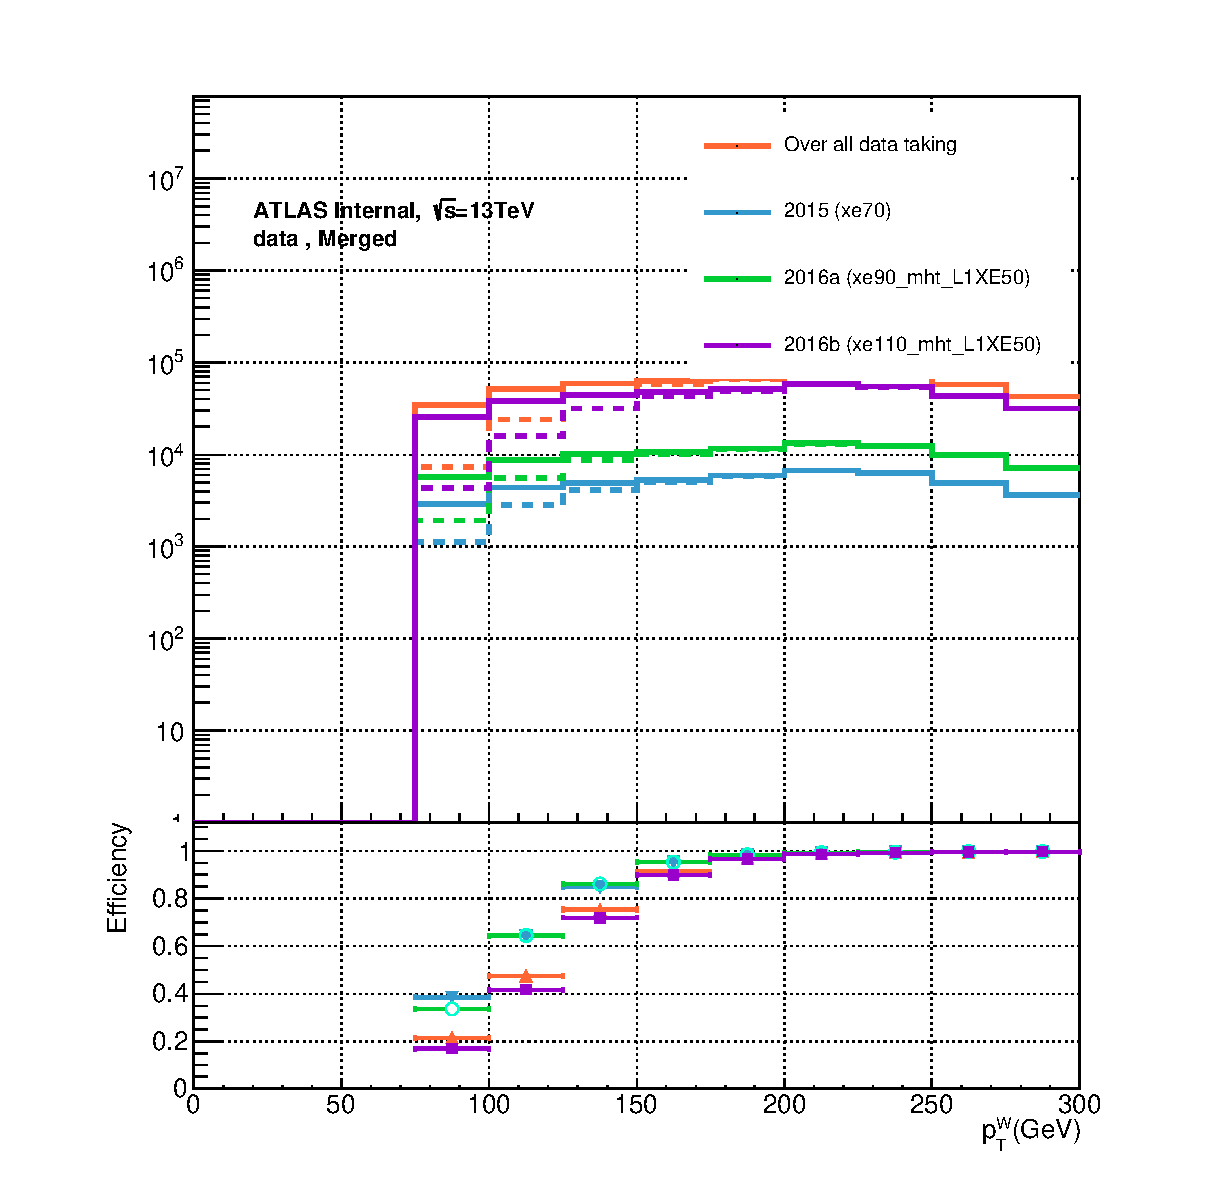
\includegraphics[width=0.48\hsize]{Chapter3/Merged_TrigEff_ptW_METcut_data.eps}
		}
		\subfloat[]{
			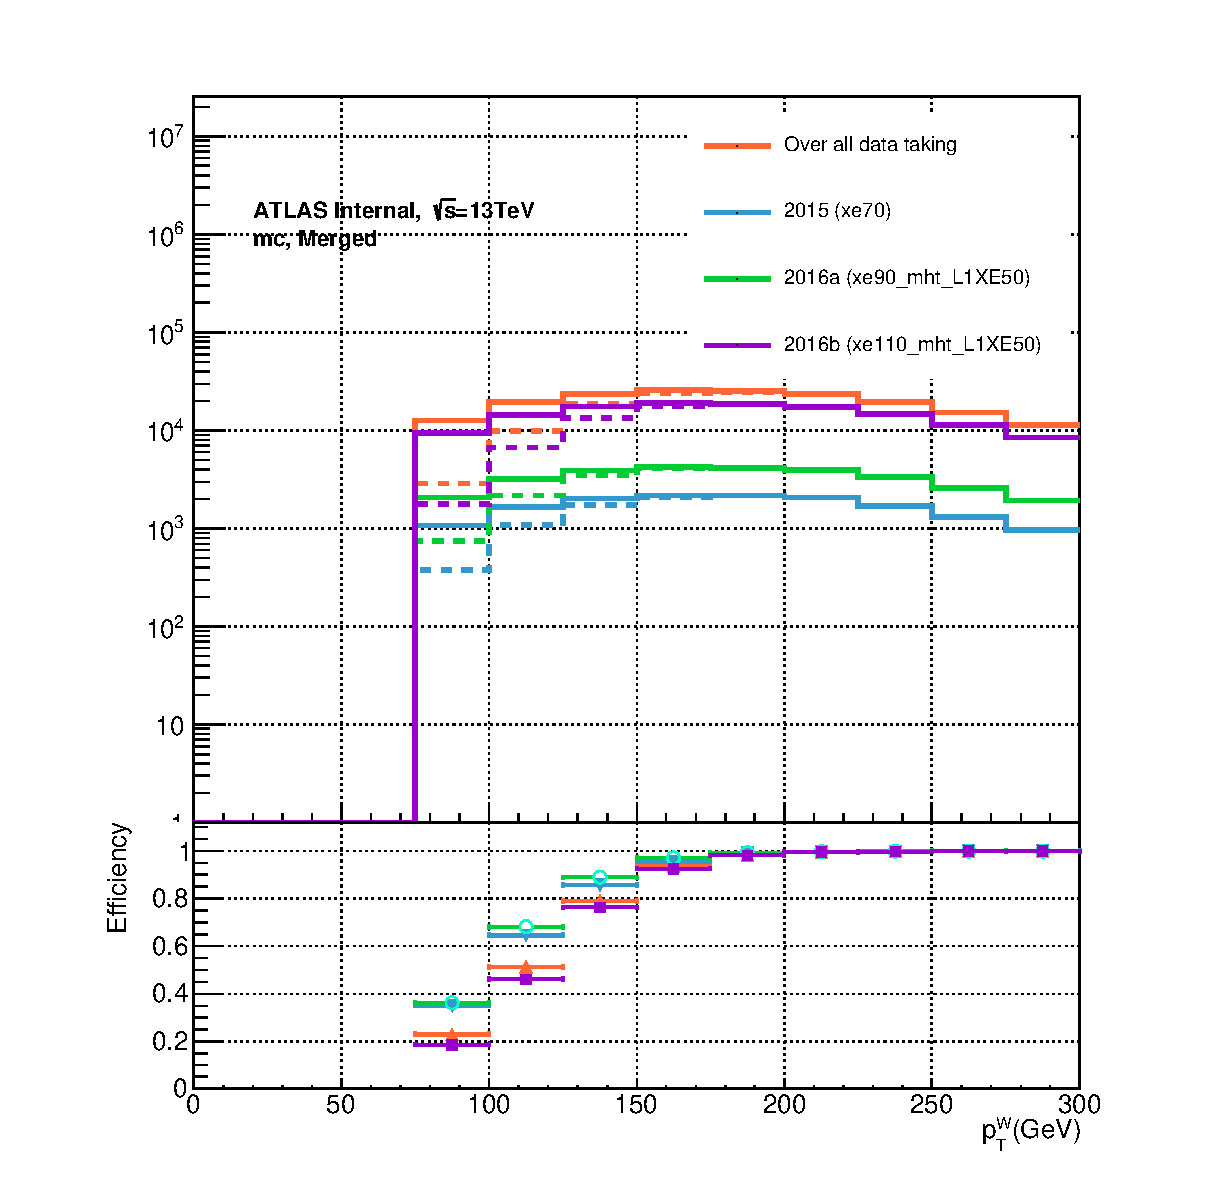
\includegraphics[width=0.48\hsize]{Chapter3/Merged_TrigEff_ptW_METcut_ttbar.eps}
		}
		\caption{The upper plot is $p_{T}(\mu\nu)$ distribution of tagged (real) and probed events in boosted channel for data (a) and $t\bar{t}$ events (b). The lower plots is the efficiency as a function of $p_{T}(\mu\nu)$}
		\label{Fig:eff_met_merged}
	\end{center}
\end{figure}

\begin{figure}[ht]
	\begin{center}
		\subfloat[]{
			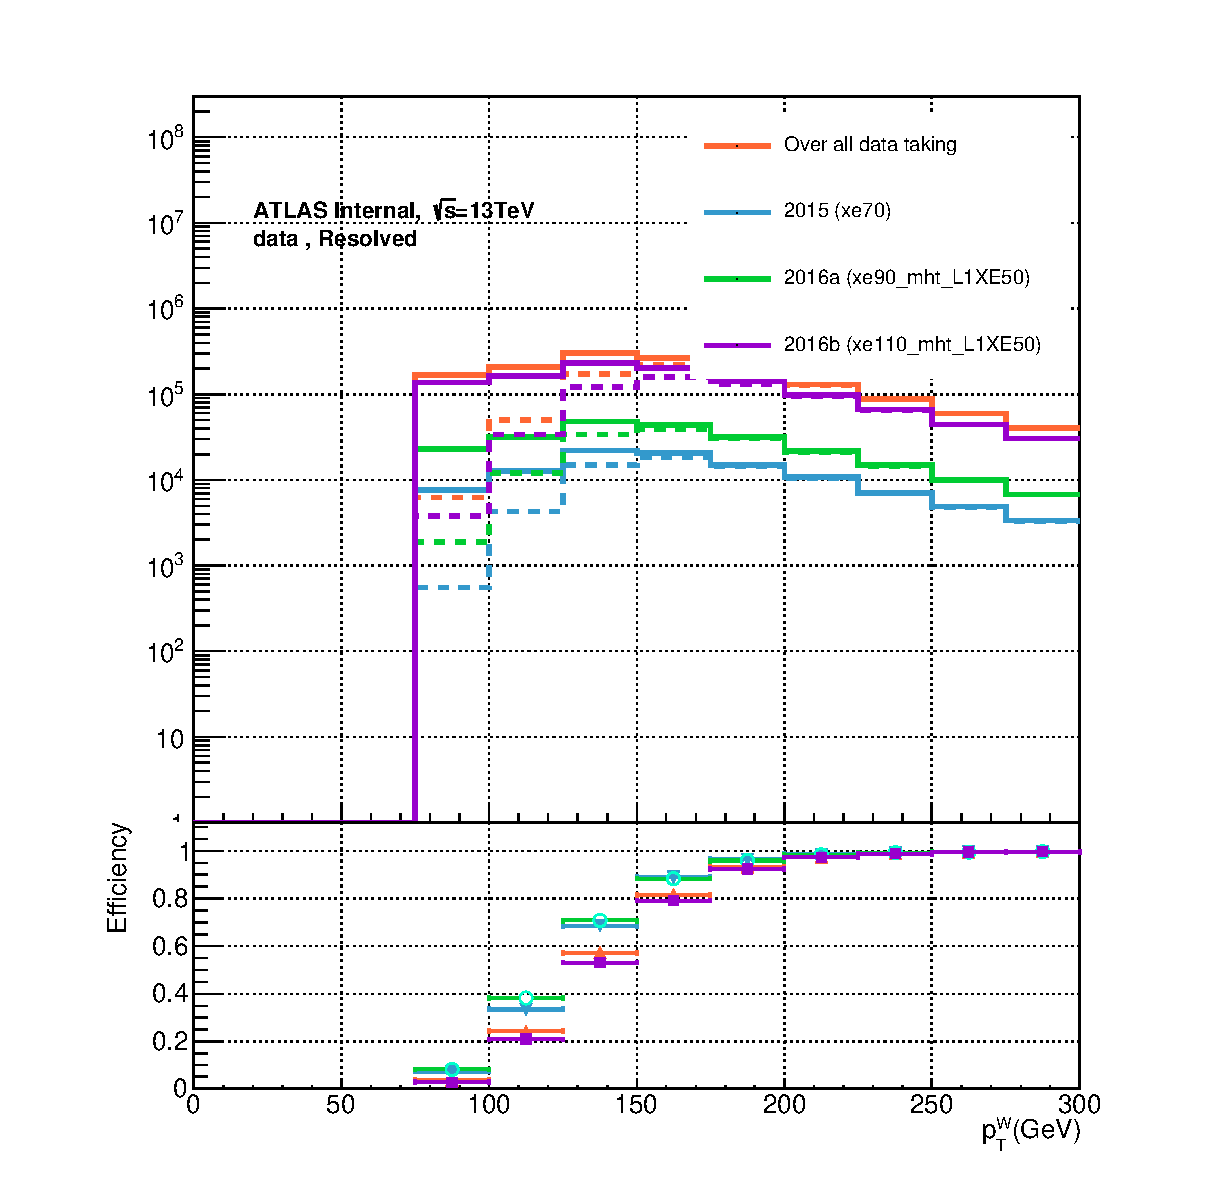
\includegraphics[width=0.4\hsize]{Chapter3/Resolved_TrigEff_ptW_METcut_data.eps}
		}
		\subfloat[]{
			\includegraphics[width=0.48\hsize]{Chapter3/Resolved_TrigEff_ptW_METcut_ttbar-eps-converted-to}
		}
		\caption{The upper plot is $p_{T}(\mu\nu)$ distribution of tagged (real) and probed events in resolved channel for data (a) and $t\bar{t}$ events (b). The lower plots is the efficiency as a function of $p_{T}(\mu\nu)$}
		\label{Fig:eff_met_resolved}
	\end{center}
\end{figure}
\noindent
\subsection{Event Cleaning and Preselection}
After the trigger, the event ``quality is verified by a series of flags in data determining the suitability of an event for physical analyses. The following is the list:
\begin{itemize}
	\item {\bf Good Run}: when the detector operates in a proper status without intolerable defects, the runs go into the good run list (GRL). Only the events contained in the GRL are considered in this analysis. 
	\item {\bf Primary Vertex}: because all the physical objects are required to origin from the primary vertex, its existence is essential. Events without a proper primary vertex (defined in Sec. \ref{sec:obj rec}) are discarded.
	\item {\bf Tile Error Veto}: part of the channels in tile detector are broken. If they accept any physical objects, this flag would be marked, and the events are vetoed.
	\item {\bf LAr Error Veto}: part of the channels in LAr detector are broken. If they accept any physical objects, this flag would be marked, and the events are vetoed.
	\item {\bf SCT Error Veto}: part of the channels in SCT detector are broken. If they accept any physical objects, this flag would be marked, and the events are vetoed.
	\item {\bf Core Error Veto}: during data-taking periods, the atlas central DAQ system might suffer from some glitches which broke the data recording, and the flag is marked for events. They are also vetoed in this analysis. 
\end{itemize}
\subsection{Parameter of Interest, $m_{WV}$}
This analysis is searching for the mass resonance of exotic particles, so it is the discriminant to seek for the signal. (i.e. $m_WV$ distribution is the input for statistic interpretation.) However, the longitudinal $p_{T}$ of neutrinos in the final state could not be measured, so the mass resolution is poor to spot the signal spike. Therefore, $p_{z}(\nu)$ is solved with the assumption that $W\rightarrow l\nu$ is the $E^{miss}_{T}$ contribution in all the events although it is not held true in every event. Firstly, the equation of energy conservation of $W$ boson decay can be written down as:
\begin{equation}
m^2_W = m_{l}^{2} + 2E_{l}\sqrt{ p_{T,\nu}^2 + p_{z,\nu}^{2} }  - 2 \vec{p}_{{T},l} \cdot \vec{p}_{T, \nu} - 2 p_{z, l} p_{z,\nu}
\end{equation}
\noindent
In SM, W bosons have the mass of $80~GeV$, so $m_{l}$ for electrons and muons is negligible. This leads to the quadratic equation of $p_{z}^\nu$:
\begin{equation}
4p_{{T}, l}^{2} p_{z,\nu}^{2} - 4 \left( m_{W}^{2} + 2 \vec{p}_{{T}, l} \cdot \vec{p}_{{T},\nu} \right) p_{z,l} p_{z, \nu} - \left( m_{W}^{2} + 2\vec{p}_{{T}, l} \cdot \vec{p}_{{T},\nu}  \right)^{2} +4p_l^{2} p_{{T},\nu}^{2} = 0
\end{equation}
\noindent
If the solutions are complex, only the real terms are taken into this analysis, and the imaginary term is discarded. To determine which solution from the real terms to use, the resolution is compared with the absolute value of solutions (bigger one and smaller one) defined as:
\begin{equation}
\sigma = \frac{p_z^{truth}-p_z^{\nu}}{p_z^{truth}}
\end{equation}
\noindent
with $p_z^{truth}$ as the neutrino longitudinal momentum at generator level (MC truth). The result could be seen in Fig. \ref{Fig:netrinoPz}, and it indicates the bigger one has slightly better performance in terms of the mass resolution, so it is kept.  
\begin{figure}
	\centering
    \includegraphics[width=0.5\hsize]{Chapter3/neutrinoPz}
    \caption{The $p_{z}^\nu$ resolution with absolute values of the solutions, bigger and smaller one. }
    \label{Fig:netrinoPz}
\end{figure}
\noindent
In addition to the correction on the leptonically decayed W boson, the other further improvement on $m_{WV}$ reconstruction is also made by $p_{T}(j,j)$ of the two resolved signal jets by the correction of $p_{T}^{corr}=p_{T}(j,j)\times \frac{m_{V}}{m_{jj}}$ (For WW, $m_V$ is taken as W boson mass, while it is Z boson mass for WZ medium state). The improvement of the ``mass-constraint'' correction could be seen in Fig. \ref{Fig:WHadmassConst} for $\approx 20\%$ better $m_{WV}$ resolution. 
\begin{figure}[h]
	\centering
	\includegraphics[width=0.6\hsize]{Chapter3/lvjjmass_WmassConstraint}
	\caption{$m_{WV}$ distributions for $gg \rightarrow H \rightarrow WW$ signals at $m=300~GeV$ (solid), 500~GeV (dashed) and 700~GeV (dot), with (red) and without (blue) $W$-mass constraint to $W \rightarrow jj$ system.}\label{Fig:WHadmassConst}
\end{figure}
\noindent
\subsection{VBF Event Selection}
As VBF signal regions have better sensitivity than ggF/DY ones, the selection criteria play an important role in this analysis. The optimization on the selection is conducted in three steps. First, all VBF events are required to have at least 4(2) jets in the resolved (boosted) channel. Second, the the two jets in the dijet system are supposed to be the pair with the highest mass, opposite $\eta$ signs, and not b-tagged. This pair was chosen prior to the $W/Z\rightarrow jj$ signal jet selection and removed from signal jet candidates. Then, the optimization is performed on a 2-dimensional phase space constructed by $\Delta\eta(j,j)$ and $m(j,j)$ which are two most evident signatures of this production process. The performance of the cuts on the two variables is determined by signal significance in Eq. \ref{Eq:significance}. Fig. \ref{Fig:VBFOptimization} shows the result of the optimization performed on the signal sample with $700~GeV$ HVT, and the best significance could be achieved by:
\begin{itemize}
	\item {\bf $m_{jj}^{VBF}> 770~GeV$}
	\item {\bf $\Delta\eta(jj)>4.7$}
\end{itemize}
The other reason to choose this set of cuts is to make it consistent with $WZ/ZZ \rightarrow lljj/\nu\nu jj$ analysis\cite{EXOT-2016-29} for the combination in next chapter. 
\begin{figure}[h]
	\centering
	\includegraphics[width=0.7\textwidth]{Chapter3/VBF700_SignfSpace}
	\caption{The signal significance for the VBF $WW$ signal as a function of the VBF cuts $\Delta \eta(j_1,j_2)$ and $m(jj)$ for signal mass 700~GeV (right). The black outlined bins are those whose values vary from the maximum by less than 5\%.}
	\label{Fig:VBFOptimization}
\end{figure}
\subsection{Boosted Event Selection}
In the boosted channel, the most important selection above the others is that at least one large R jet fulfils the W/Z boson $80\%$ efficiency tagging working points. Then, those events are further categorized into high purity and low purity regions determined by whether the 50$\%$ tagging working points are passed. The full selection is seen in Tab.~\ref{tab:SRdefinitions}. It should be noted that W and Z boson taggers are applied respectively in signal regions to separate the $W\to J$ and $Z\to J$ events, which gives the WW and WZ signal regions for each signal region category. 

\begin{table}[t]
	\caption{Summary of the selection criteria in the definition of the signal region (SR), $W$+jets control region ($W$ CR) and $t\bar{t}$ control region ($t\bar{t}$ CR), in the high-purity (HP) and low-purity (LP) categories.  } \label{tab:SRdefinitions}
	\begin{center}
		\begin{adjustbox}{center}
		\begin{tabular}{|l|l|c|c|c|c|c|c|}
			\hline
			\multicolumn{2}{|l|}{\multirow{2}{*}{Selection}} & \multicolumn{2}{c|}{SR}  &  \multicolumn{2}{c|}{$W$ CR}  & \multicolumn{2}{c|}{$t\bar{t}$ CR} \\
			\cline{3-8}
			\multicolumn{2}{|l|}{} & HP & LP &HP & LP & HP & LP \\
			\hline
			\multirow{4}{*}{$W\rightarrow l\nu$} & Num of signal leptons & \multicolumn{6}{c|}{ 1 } \\
			\cline{2-8}
			&Num of vetoed leptons & \multicolumn{6}{c|}{ 0 }  \\
			\cline{2-8}
			&\vphantom{\Large B} $E^{miss}_{T}$ & \multicolumn{6}{c|}{ $>100GeV$ } \\
			\cline{2-8}
			&$p_{T}(l\nu)$ & \multicolumn{6}{c|}{ $>200GeV$ } \\
			\hline
			\multirow{5}{*}{$W/Z\rightarrow J$} & Num of large-$R$ jets & \multicolumn{6}{c|}{ $\geq 1$ } \\
			\cline{2-8}
			& \vphantom{\Large B} $D^{(\beta=1)}_2$ 50\,\% WP & pass & fail & pass & fail & pass & fail \\
			\cline{2-8}
			& \vphantom{\Large B} $D^{(\beta=1)}_2$ 80\,\% WP & --- & pass  & --- & pass  & --- & pass \\
			\cline{2-8}
			& $W/Z$ mass 50\,\% WP & pass &fail& --- & --- & pass & fail\\
			\cline{2-8}
			& $W/Z$ mass 80\,\% WP &  --- & pass & fail & fail & --- & pass\\
			\hline
			\multirow{2}{*}{Topology cuts}
			& $p_{T}(l\nu) / m_{WV}$ & \multicolumn{6}{c|}{ \multirow{2}{*}{$>0.3 (0.4)$ for VBF (ggF) category } }\\
			& $p_{T}(J) / m_{WV}$  & \multicolumn{6}{c|}{} \\
			\hline
			Top-quark veto & Num of $b$-tagged jets & \multicolumn{4}{c|}{0} & \multicolumn{2}{c|} {$\geq 1$} \\
			\hline
			Multi-jet BG Cleaning Cut & $E_T^{miss} / p_T(lv) > 0.2$ & \multicolumn{6}{c|}{ Electron channel only } \\
			\hline
			\multicolumn{2}{|c|}{Existence of VBF jets} & \multicolumn{6}{c|}{ yes (no) for VBF (ggF) category } \\
			\hline
		\end{tabular}
	    \end{adjustbox}
	\end{center}
\end{table}
\noindent
\\For the other boson system which decays leptonically, the requirement is that exactly one signal lepton is selected with $E^{miss}_{T}$ above $100~GeV$ to suppress the multijet background. The additional requirements on the leptonical decay system is two topological cuts with the study on the simulation samples: 
\begin{itemize}
	\item[] (a) $E^{miss}_{T}/p_{T}(e,\nu)>0.2$
	\item[] (b) $p_{T}(\ell,\nu)/m_{WV}>0.3(0.4)$ for VBF (ggF) category
\end{itemize}
(a) is only for the electron channel to reduce multijet background of which electrons and $\met$ are irrelevant, so the events tend to have smaller ratio of $met$ over $p_{T}(e,\nu)$ (transverse vector sum of $met$ and electron $p_T$). For the case of (b), because the two reconstructed bosons in SM background events are not correlated, the ratio of $p_{T}(ell, \nu)$ over $m_{WV}$ has smaller number. Therefore, the cut is deployed to suppress the SM background contribution.\cite{EXOT-2016-28} These criteria are consistent across signal and control regions. 
\\
\\On the side of the hadronically decayed boson is only the large R jet. In addition to the requirement in the last section, the high purity regions (HP) (for both signal and control regions) demand the fat jet boson-tagged at $50\%$ WP, and it is the most sensitive region to signal. Events with fat jets failing $50\%$ but passing $80\%$ WPs go into the low purity region (LP). By doing this, the combined sensitivity of the HP and LP signal regions is improved by around $~10\%$.\cite{EXOT-2016-28} If the fat jet only fails mass cut and pass the $D_{2}^{\beta=1}$ of boson tagging, this event would not be discarded but chosen into W+jet control region instead. Finally, $p_{T}$ of the fat jet is also required to be above $0.3(0.4)m_{WV}$ for the energy balance in VBF(ggF) category. The event categorization of signal and W+jet control regions for both high and low purity categories is illustrated in Fig.~\ref{Fig:HPLPdefinitions}.
\begin{figure}[h]
	\centering
	\includegraphics[width=0.8\hsize]{Chapter3/HPLPdefinitions}
	\caption{Definitions of signal region (SR) and $W$+jets control region (CR) for the event with the large-R jet of $\pt=1\,\TeV$ based on fat jet boson tagging parameters, $D_{2}^{\beta=1}$ and fat jet mass. }
	\label{Fig:HPLPdefinitions}
\end{figure}
\noindent
To reduce the $t\bar{t}$ background contribution, the subjets associated to the selected large R jet shall not be b-tagged in the W+jet control region and signal region. If any of them or the small R jets ($R=0.4$) pass the $85\%$ b-tagging WP, the event would go into the top control region. 
\\
\\Fig.~\ref{Fig:HighPuritySR} and Fig.~\ref{Fig:LowPuritySR} are the $m_{WV}$ distributions for the comparison of signal and background events in high purity and low purity signal regions for electron and muon channels respectively. 
\begin{figure}[h]
	\begin{center}
		\subfloat[]{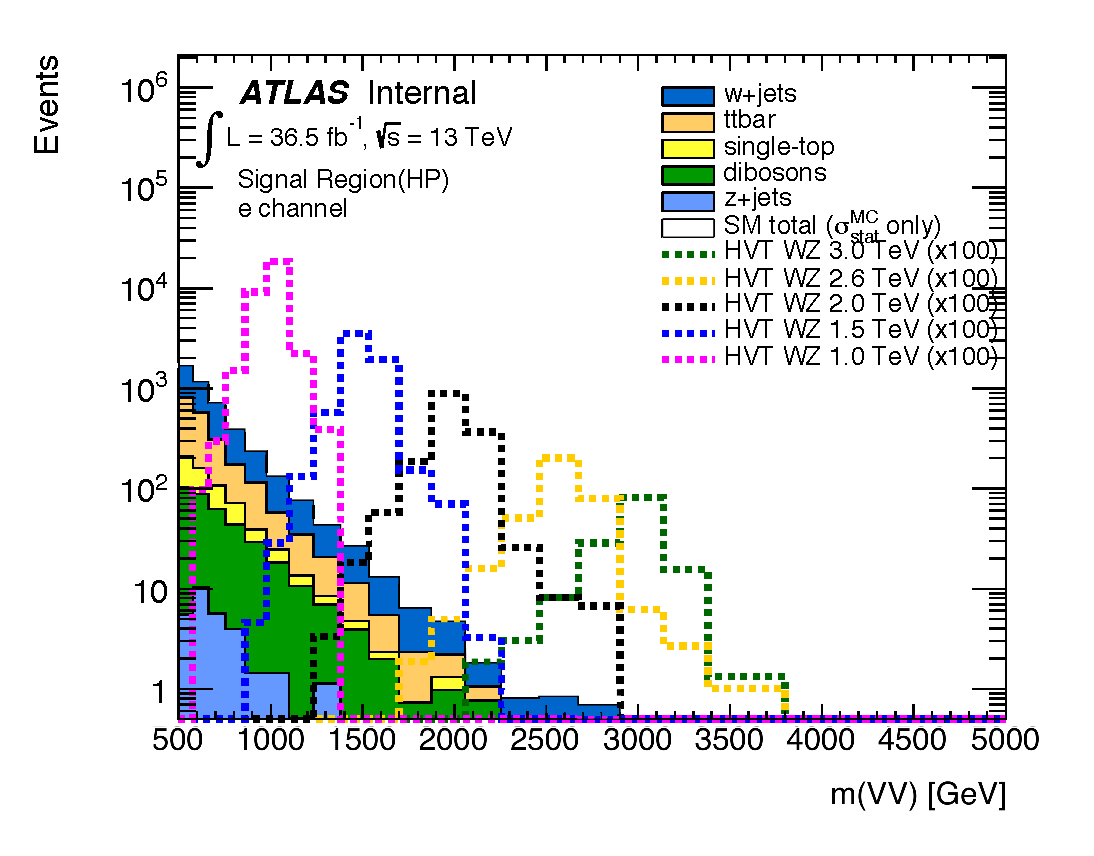
\includegraphics[width=0.5\hsize]{Chapter3/lvJmass_bveto_e.eps}}
		\subfloat[]{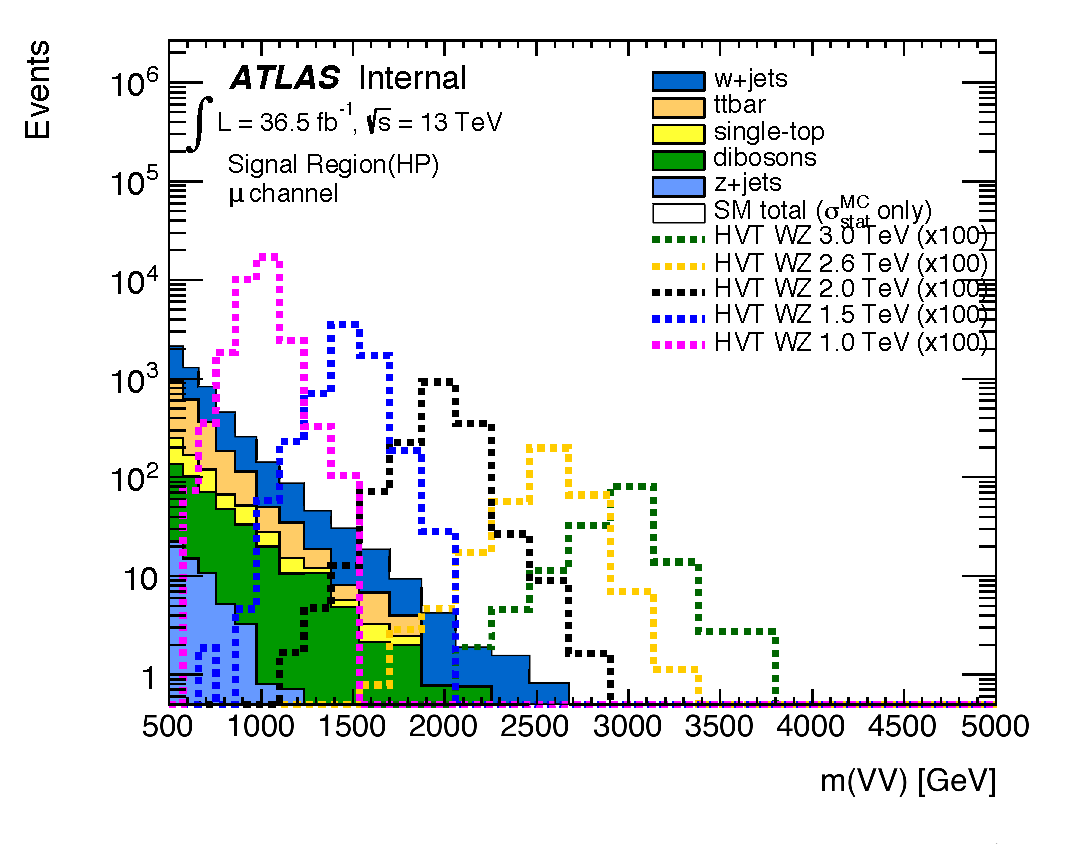
\includegraphics[width=0.5\hsize]{Chapter3/lvJmass_bveto_mu.eps}}
	\end{center}
	\caption{The $m_{WV}$ distribution (denoted as m(VV) in the plots) in the HP signal region for (a) electron and (b) muon channels for SM background from simulation which is normalized to the integrated luminosity of $36.5~fb^{-1}$.The HVT $WZ$ signals with mass of $1.0~TeV$, $1.5~TeV$, $2.0~TeV$, $2.6~TeV$ and $3.0~TeV$ are overlaid and
		scaled to $100 ~\times$ the cross section.}
	\label{Fig:HighPuritySR}
\end{figure}

\begin{figure}[h]
	\centering
	\subfloat[]{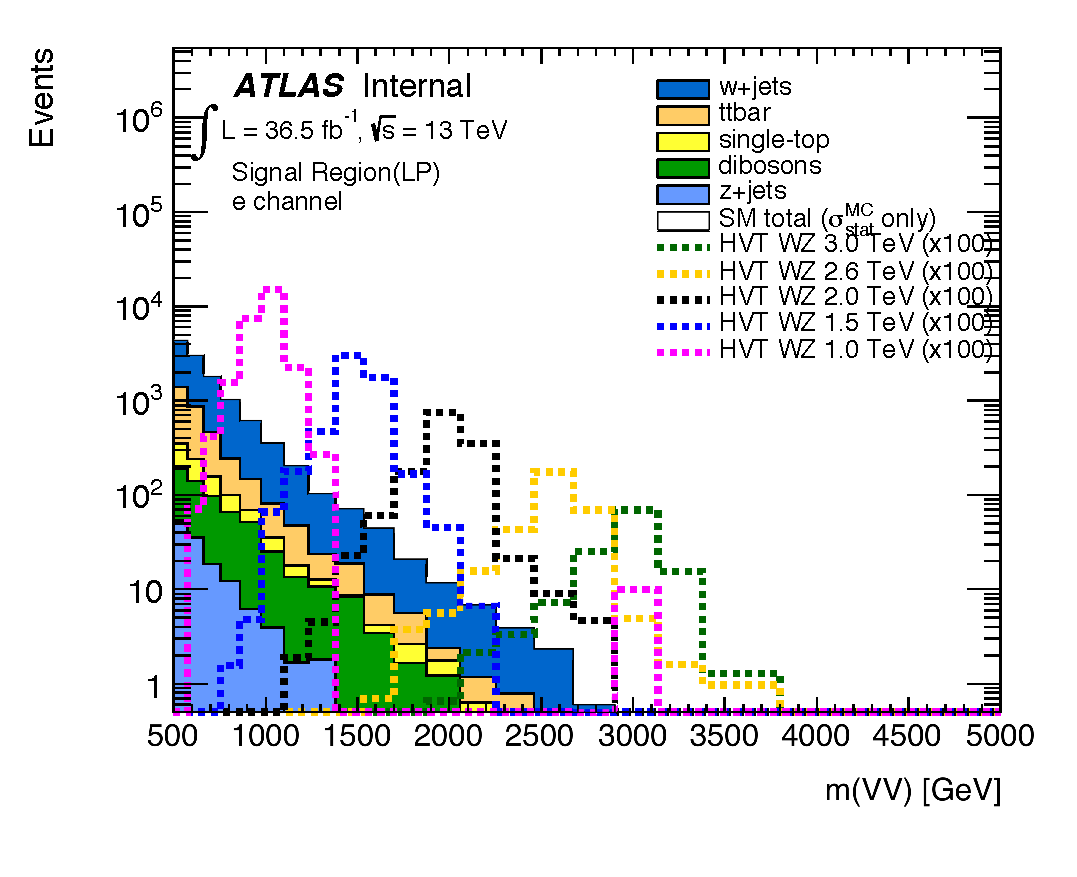
\includegraphics[width=0.5\hsize]{Chapter3/lvJmass_lowPurity_e.eps}}
	\subfloat[]{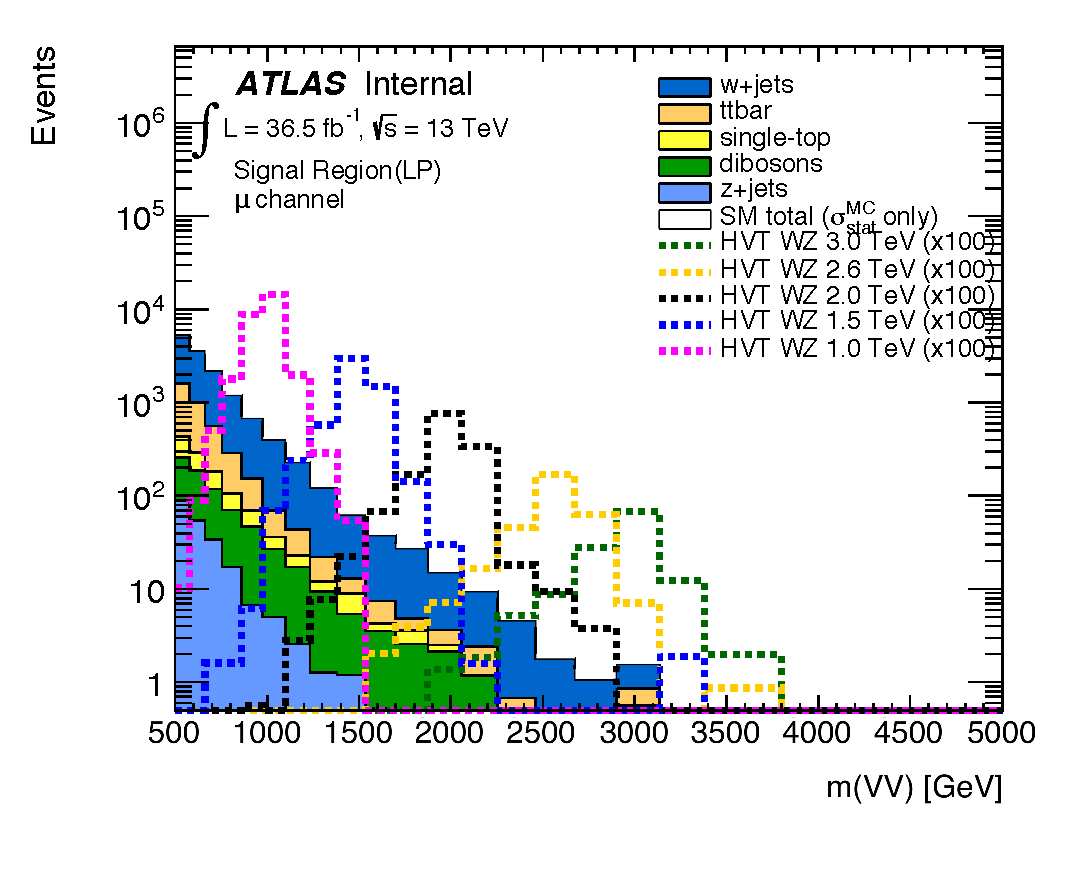
\includegraphics[width=0.5\hsize]{Chapter3/lvJmass_lowPurity_mu.eps}}
	\caption{The $m_{WV}$ distribution (denoted as m(VV) in the plots) in the LP signal region for (a) electron and (b) muon channels for SM background from simulation which is normalized to the integrated luminosity of $36.5~fb^{-1}$.The HVT $WZ$ signals with mass of $1.0~TeV$, $1.5~TeV$, $2.0~TeV$, $2.6~TeV$ and $3.0~TeV$ are overlaid and
	scaled to $100 ~\times$ the cross section.}
	\label{Fig:LowPuritySR}
\end{figure}
%

\subsection{Resolved Event Selection}
The resolved channel has a lower sensitivity than the boosted channel, but it still helps to recover the events lost in the lower energy regime. If the event has no fat jet fulfilling the selection criteria, it goes to the resolved category. The full selection for resolved signal and control regions can be seen in Tab.~\ref{Tab:SRdefinitions_resolved}. 
\begin{table}[t]
	\caption{Summary of the selection criteria of the resolved analysis for the $WW$ and $WZ$ signal regions (SR), $W$+jets control region (WR) and $ t\bar{t}$ control region (TR). } \label{Tab:SRdefinitions_resolved}
	\begin{center}
		\resizebox{\textwidth}{!}{
			\begin{tabular}{|l|l|c|c|c|c|}
				\hline
				\multicolumn{2}{|l|}{cuts} & $WW$ SR & $WZ$ SR & WR & TR \\
				\hline
				\multirow{3}{*}{$W\rightarrow \ell\nu$ selection} & Number of signal leptons & \multicolumn{4}{c|}{ 1 } \\
				\cline{2-6}
				&Number of veto leptons & \multicolumn{4}{c|}{ 0 }  \\
				\cline{2-6}
				&$E^{miss}_{T}$ & \multicolumn{4}{c|}{ $>60GeV$ } \\
				\cline{2-6}
				&$\pt(\ell\nu)$ & \multicolumn{4}{c|}{ $>75GeV$ } \\
				\hline
				\multirow{4}{*}{$W/Z\rightarrow jj$ selection} & Number of small jets & \multicolumn{4}{c|}{ $\geq2$ } \\ %$\geq 2$ & $\geq 2$ & $\geq 2$  \\
				\cline{2-6}
				& $\pt (j1)$ & \multicolumn{4}{c|}{ $>60$~GeV}\\
				\cline{2-6}
				& $\pt (j2)$ & \multicolumn{4}{c|}{ $>45$~GeV}\\
				\cline{2-6}
				& $m_{jj}$ & [66, 94]GeV\ & [82, 106]GeV\ & $<66GeV$ &  [66, 106]GeV \\
				&  &  &  & or [106, 200]GeV & \\
				\hline
				\multirow{6}{*}{Topology cuts} & $\Delta\phi(j,\ell)$ & \multicolumn{4}{c|}{ $>1.0$}\\
				\cline{2-6}
				& $\Delta\phi(j,E^{miss}_{T})$ & \multicolumn{4}{c|}{ $>1.0$}\\
				\cline{2-6}
				& $\Delta\phi(j,j)$ & \multicolumn{4}{c|}{ $<1.5$}\\
				\cline{2-6}
				& $\Delta\phi(l,E^{miss}_{T})$ & \multicolumn{4}{c|}{ $<1.5$}\\
				\cline{2-6}
				& $\pt(e\nu) / m_{WV}$ &\multicolumn{4}{c|}{\multirow{2}{*}{$>0.3 (0.35)$ for VBF (ggF) category}}\\
				& $\pt(jj) / m_{WV}$ & \multicolumn{4}{c|}{ } \\
				\hline
				\multirow{2}{*}{Top veto} & Number of $b$-tagged jets in $W/Z$ & $\leq 1$ & $\leq 2$ & $\leq 1$ & $\geq2$ \\
				\cline{2-6}
				& Number of other $b$-tagged jets & \multicolumn{3}{c|}{0} & or $\geq 1$ \\
				\hline
				\multicolumn{2}{|c|}{Existence of VBF jets} & \multicolumn{4}{c|}{ yes (no) for VBF (ggF) category } \\
				\hline
			\end{tabular}
		}
	\end{center}
\end{table}
\noindent
\\As in the boosted channel, the leptonically decaying W boson has a signal lepton fulfilling the object definition of the last section. However, the $E_{T}^{miss}$ cut here is lowered to $60~GeV$ for the less energetic system as compared to the boosted channel. For the energy balance, the ratio between $p_{T}(l,\nu)$ and $m_{WV}$ shall be over 0.3 (0.35) for VBF (ggF) category. 
\\
\\On the hadronic side, the two signal jets are selected after VBF jets, and they are required to have $p_{T}$ above $60~GeV$ ($45~GeV$) for the leading (subleading) one to suppress the SM background. Similar to the boosted event selection, to recognize the boson which decays to the two jets, two mass windows are applied respectively to select WW and WZ signal regions, which are $[66, 94]~GeV$ for WW signal region ($W\to jj$) and $[82, 106]~GeV$ for the WZ signal region ($Z\to jj$). The top control regions don't have the WW and WZ regions separated, so the mass window is applied with $[66,106]~GeV$ as the OR condition of W and Z mass windows. Events with a dijet mass which falls into the side band region of W and Z boson mass ($[0,66]~GeV$ or $[106,200]~GeV$) are taken into the W+jet control region. The energy balance requirement here is the same as the leptonic system: $p_{T}(jj)/m_{WV}>0.3(0.35)$ for the VBF (ggF) category. The two selected jets in the W(Z) mass window are allowed to have one(two) of them b-tagged. The existence of any additional b-tagged jets would then make the event go into the top control region.  
\\
\\Different from the boosted channel, the resolved channel has the abundant background contribution from multijet events (details in next section), so they are suppressed by a series of topological cuts with the optimization by the study on the dijet MC samples, which are listed below \cite{EXOT-2016-28}:
\begin{itemize}
	\item $\Delta\phi(j,l)>1.0$
	\item $\Delta\phi(j,\met)>1.0$
	\item $\Delta\phi(j,j)<1.5$
	\item $\Delta\phi(l,\met)<1.5$
\end{itemize}
\noindent
\\Fig.~\ref{Fig:ResolvedSR} is the $m_{WV}$ distributions for comparison of signal and background in resolved signal regions for ggF and VBF categories respectively. The signal samples are with lower mass, because resolved channel has better sensitivity to them. 
\begin{figure}[h]
	\centering
	\subfloat[]{\includegraphics[width=0.5\hsize]{Chapter3/lvjjmass_ggF}}
	\subfloat[]{\includegraphics[width=0.5\hsize]{Chapter3/lvjjmass_VBF}}
	\caption{The $m_{WV}$ (denoted as m(VV) in the plots) distribution in the resolved signal region for (a) ggF and (b) VBF channels for SM background from simulation which is normalized to the integrated luminosity of $36.5~fb^{-1}$.The HVT $WZ$ signals with mass of $300~GeV$, $500~GeV$, and $700~GeV$ are overlaid and
		scaled to $100 ~\times$ the cross section..}
	\label{Fig:ResolvedSR}
\end{figure}

\subsection{Multijet Background Estimation}
\label{sec:multijet_background}
As discussed above, the SM backgrounds are estimated from Monte-Carlo simulation and constrained in the dedicated control regions. However, multijet processes is poorly modelled due to the lack of understanding to QCD, so simulation is not feasible for this background contribution. Its contribution is from the following sources:
\begin{itemize}
	\item {\bf Photon Conversion}: When photons or pions interact with the detector material, they decay to soft leptons with similar behaviour to signal ones, which is difficult to recognize. This contribution is mainly into electron, while it could be suppressed by combined muon requirement in muon channel
	\item {\bf Lepton Misidentification}: Soft charged partons could be blocked at ECAL and leave no signature in HCAL, which is identical to electron signatures. In this case, they are reconstructed as electrons instead of jets. This source only contributes to electron channel.
	\item {\bf Heavy Hadron Decay}: The decay products of heavy partons also include leptons. If their decay is close to the primary vertex, the decayed leptons are not distinguishable from the prompt ones. Both electrons and muons have the contribution from this source. 
\end{itemize}
\noindent
As an alternative, the estimation is performed with fake factor method, a data-driven approach. It is only significant in resolved channel while begin negligible in boosted channel.  The details of this method could be found in the ATLAS Run2 VHbb analysis~\cite{ATLAS-CONF-2016-091, ATL-COM-PHYS-2016-429}. 

\subsubsection*{Methodology}

In the method, to be orthogonal to the signal and control region, fake factors are estimated in the region with only one small R jet called single jet control region where the existence of fat jet passing the selection is not allowed ($p_{T}^{J}>200GeV$ \&\& $m^{J}>50GeV$) to keep the orthogonality to boosted region. This region is then further divided into two subregions by lepton isolation, as shown in table \ref{tab:LepIsoCR}. With $p_{T}(\mu\nu)<150 GeV$, an isolated muon trigger is applied with quality, $ivarmedium $, so the isolation requirement for inverse muon is tightened to remove the bias. As region $p_{T}(\mu\nu)>150 GeV$ is using $E_{T}^{miss}$ trigger, so the isolation bias is not presents. Fake factors in the dedicated bins are defined as:
\begin{equation}
 f = \frac{N_{event}(SingleJetSigLepCR)}{N_{event}(SingleJetInvLepCR)}
\end{equation}
with the binning in Table~\ref{tab:FFBinning}. Fake factors have the dependence on lepton eta (this dependence is for the consideration of detector homogeneity) and $p_{T}$. Additional binning on $E_{T}^{miss}$ is applied in electron channel. For both channels, fake factor is estimated in two different regions with $p_{T}(\mu\nu)<150 GeV$ and $p_{T}(\mu\nu)>150 GeV$ to achieve better precision. Fake factor is shown as a function of lepton $p_{T}$ in Figure~\ref{fig:fakefactor} for the region of $p_{T}(l\nu)>150 GeV$. It could be noticed that fake factor for electron channel is just up to $p_{T}=190GeV$. For better accuracy, the fake factor for high $p_{T}$ electron is roughly evaluated in $p_{T}$ bins only which is shown in Figure~\ref{fig:fakefactor_el_highPt}.

\begin{table}[h]
  \caption{Isolation for leptons in the single jet control region} \label{tab:LepIsoCR}
  \begin{center}

    \begin{tabular}{ | c | c | c | }
     \hline
                               &   SingleJetSigLepCR   & SingleJetInvLepCR \\ \hline
    electron                   &        TightLH        & MediumLH (!TightLH) \\ \hline
    muon($p_{T}(l\nu)>150 GeV$) &  $Iso_{trk}<0.06$    & $0.06<Iso_{trk}<0.15$ \\ \hline
    muon($p_{T}(l\nu)<150 GeV$) &  $Iso_{trk}<0.06$    & $0.06<Iso_{trk}<0.07$ \\ \hline
\end{tabular}
\end{center}
\end{table}


\begin{table}[h]
  \caption{Binning for electrons and muons to evaluate fake factor} \label{tab:FFBinning}
\begin{center}

\begin{tabular}{ | c | c | c | c |}
    \hline
    channel  & $p_{T}(GeV)$ & $|\eta|$ & $E_{T}^{miss}(GeV)$ \\ \hline
    electron & 27-115 &  & 0, 60, 75, $\infty$ \\
             & 115-135&0, 1.37, 1.52, 2.47 & 0, 38, 52, $\infty$ \\
             & 135-155& & 0, 26, 43, $\infty$ \\
             & 155-190& & 0, 25, 45, $\infty$ \\ \hline
    muon     & 27, 42, 59, 76, 99, $\infty$ & 0, 1.05, 1.5, 2.5 & N/A \\ \hline

\end{tabular}
\end{center}
\end{table}

\begin{figure}[ht]
       \centering
       \subfloat[]{\includegraphics[width=0.4\textwidth]{Chapter3/fakefactor_el_medium_highpTW}}
       \subfloat[]{\includegraphics[width=0.4\textwidth]{Chapter3/fakerate_mu_ewk}} \\
       \caption{Fake factors for the corresponding binnings (shown in text) in electron (a) and muon (b) channels}
       \label{fig:fakefactor}
\end{figure}

\begin{figure}[ht]
       \centering
       \subfloat[]{\includegraphics[width=0.4\textwidth]{Chapter3/fakerate_el_highPt.pdf}}
       \caption{Fake factors for high $p_T$ electrons}
       \label{fig:fakefactor_el_highPt}
\end{figure}


\subsubsection*{Electroweak Subtraction}

Electroweak interactions ($t\bar{t}$, W/Z+jets, diboson and single top) could also contribute to multijet events in addition to the multijet background, so they might be double counted from fake factor estimation and Monte Carlo simulation. To avoid this issue, those events are removed by employing fake factor estimation on Monte Carlo samples, which could be expressed as the following equation:
\begin{equation}
 N^{MJ}_{events} = N^{data}_{events}-N^{MC}_{event}
\end{equation}
Unfortunately, it is observed that the multijet behavior is not well-modeled in simulation with $E_{T}^{miss}>150 GeV$ for SM backgrounds. This is verified in dijet inversed lepton control region with lepton isolation inversed and at least two jets with $P_{T}>20GeV$. Figure~\ref{fig:dijetFakeCR_el} and Figure~\ref{fig:dijetFakeCR_mu} show the discrepancy between data and electroweak interactions which are contributed from multijet events. It is anticipated that multijet contribution shall be almost 0 in high $E^{miss}_{T}$ region in the dijet control region, but the discrepancy is still observed. In this case, the electroweak subtraction is applied with a scale factor derive from the ratio of events from data and simulation in the bin $150 GeV<E^{miss}_{T}<250GeV$ defined as: 
\begin{equation}
f = \frac{N_{event}(data)}{N_{event}(MC)}
\end{equation}
It is applied as an additional correction on fake factor for events with $E_{T}^{miss}>150 GeV$ from simulation. The electroweak subtraction factors for electron and muon channels are shown in Table~\ref{tab:ewsubtraction}.

\begin{figure}[ht]
       \centering
       \subfloat[]{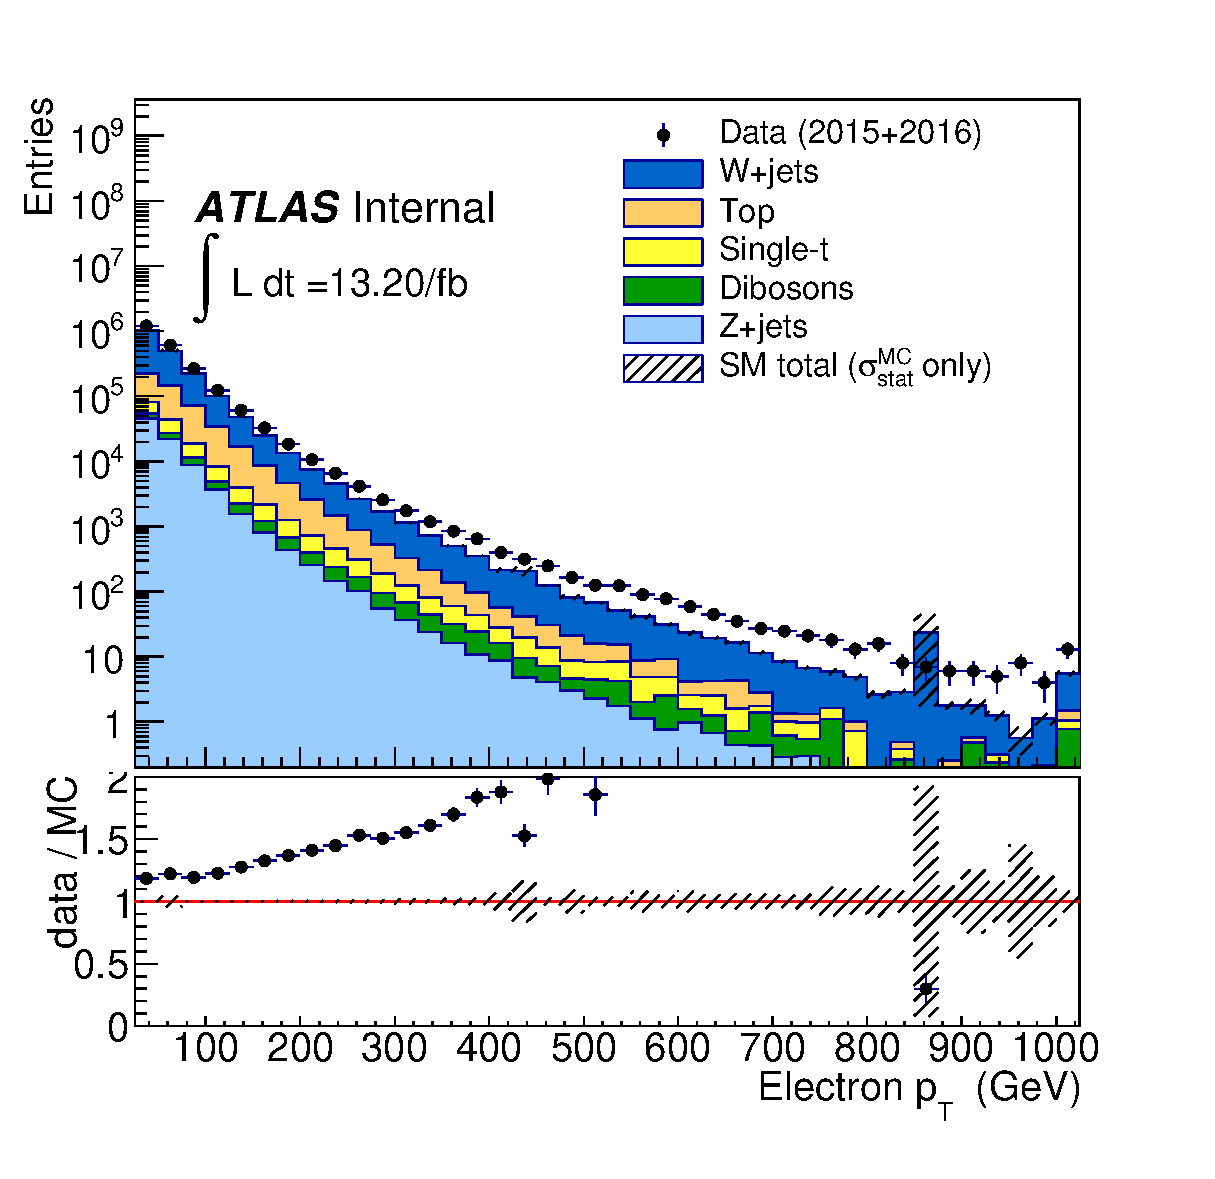
\includegraphics[width=0.45\textwidth]{Chapter3/MJ_CR/electronPt.eps}}
       \subfloat[]{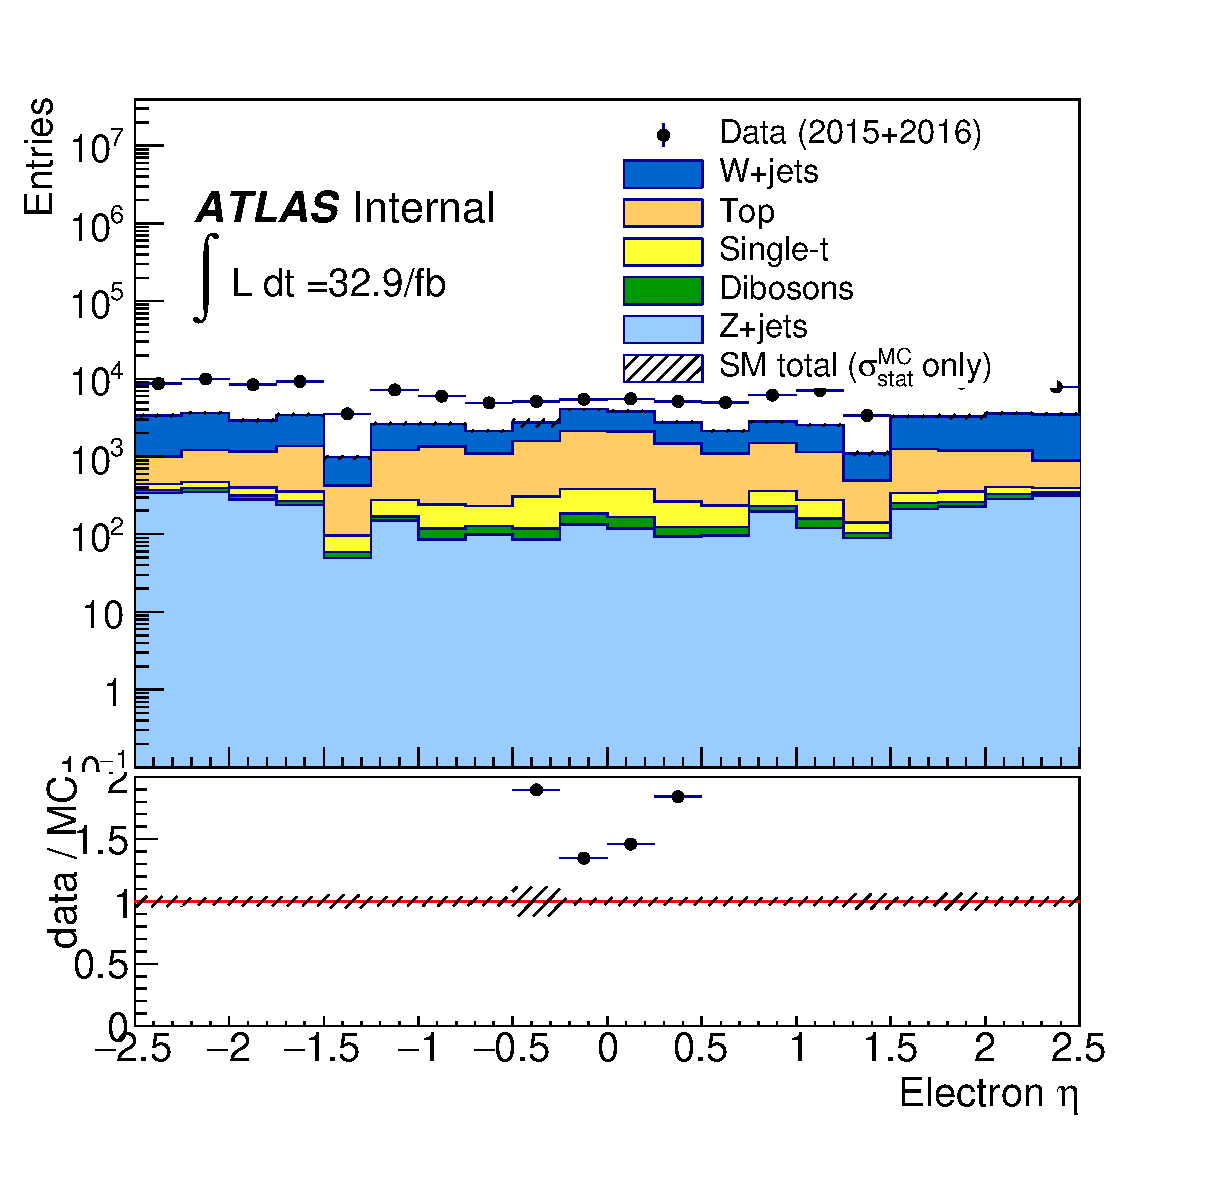
\includegraphics[width=0.45\textwidth]{Chapter3/MJ_CR/electronEta.eps}}\\ 
       \subfloat[]{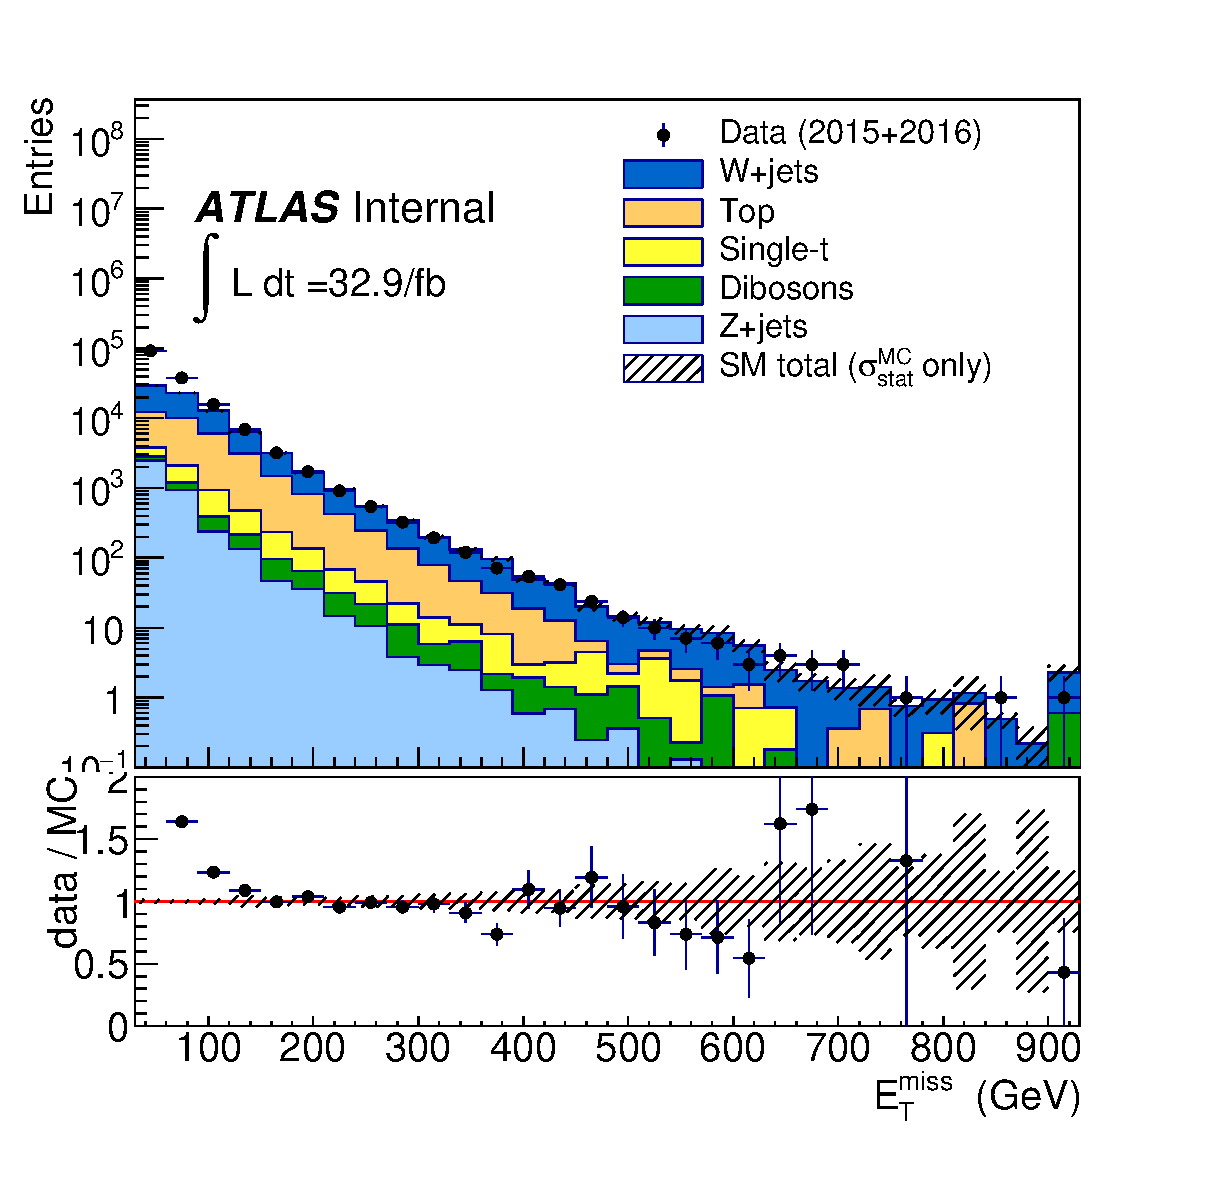
\includegraphics[width=0.45\textwidth]{Chapter3/MJ_CR/met_el.eps}}
       \subfloat[]{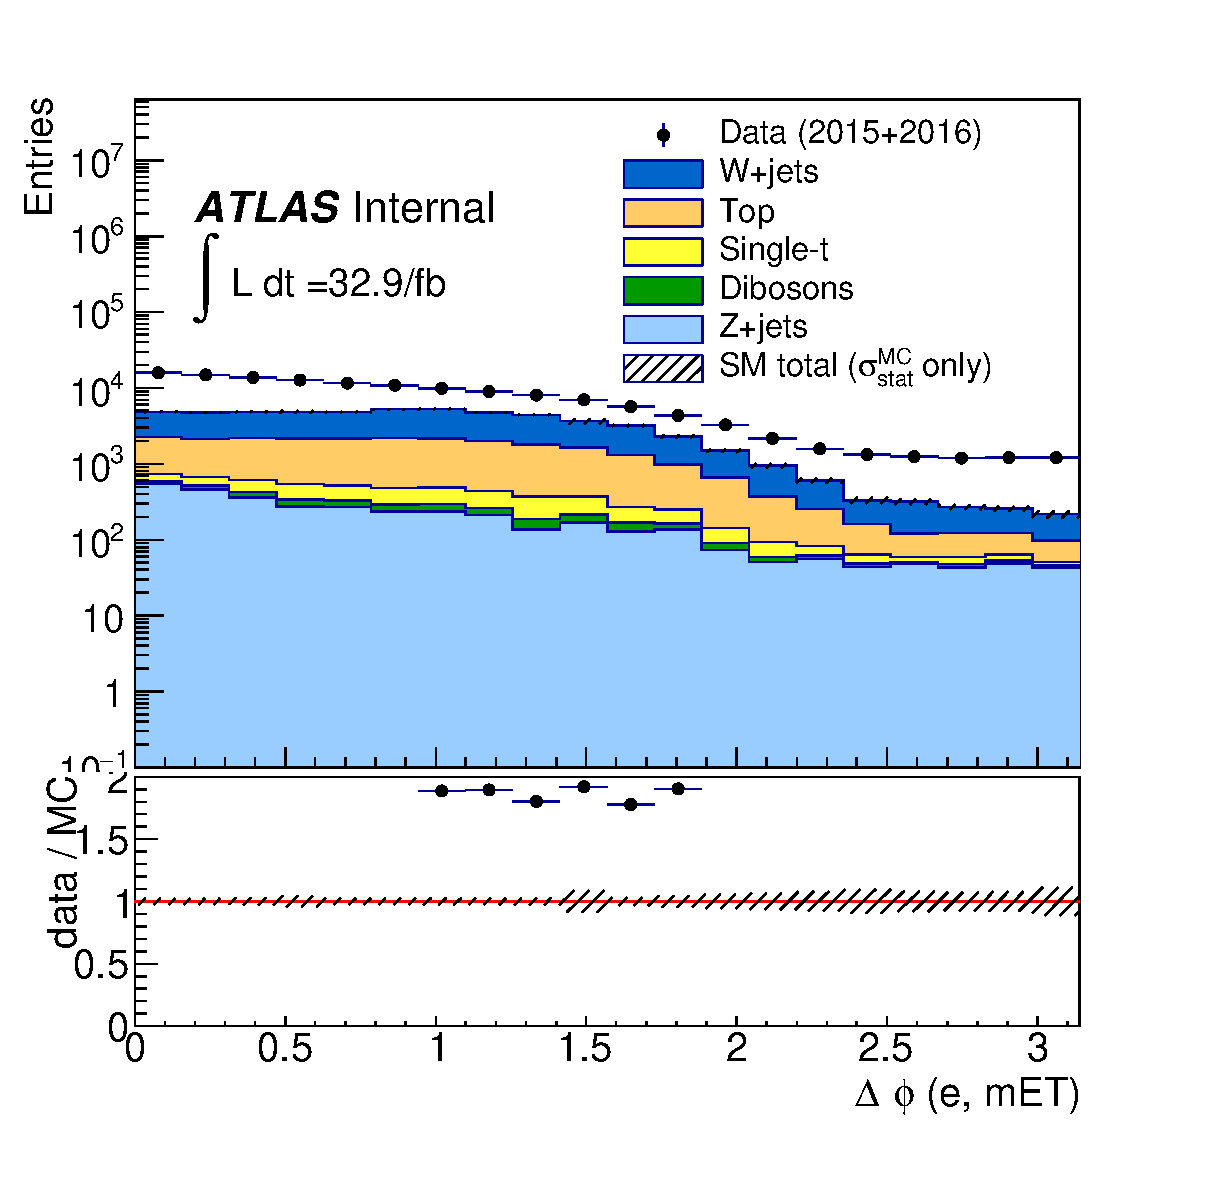
\includegraphics[width=0.45\textwidth]{Chapter3/MJ_CR/dphilepmet_el.eps}}\\
       \caption{The distribution of lepton $p_{T}$,$\eta$, $E_{T}^{miss}$ and $\Delta\phi$(e,$E_{T}^{miss}$) in dijet fake control region with inversed lepton for electron channel. The inconsistency is thought to be comprised of multijet events without applying electroweak subtraction.} 
       \label{fig:dijetFakeCR_el}
\end{figure}

\begin{figure}[ht]
       \centering
       \subfloat[]{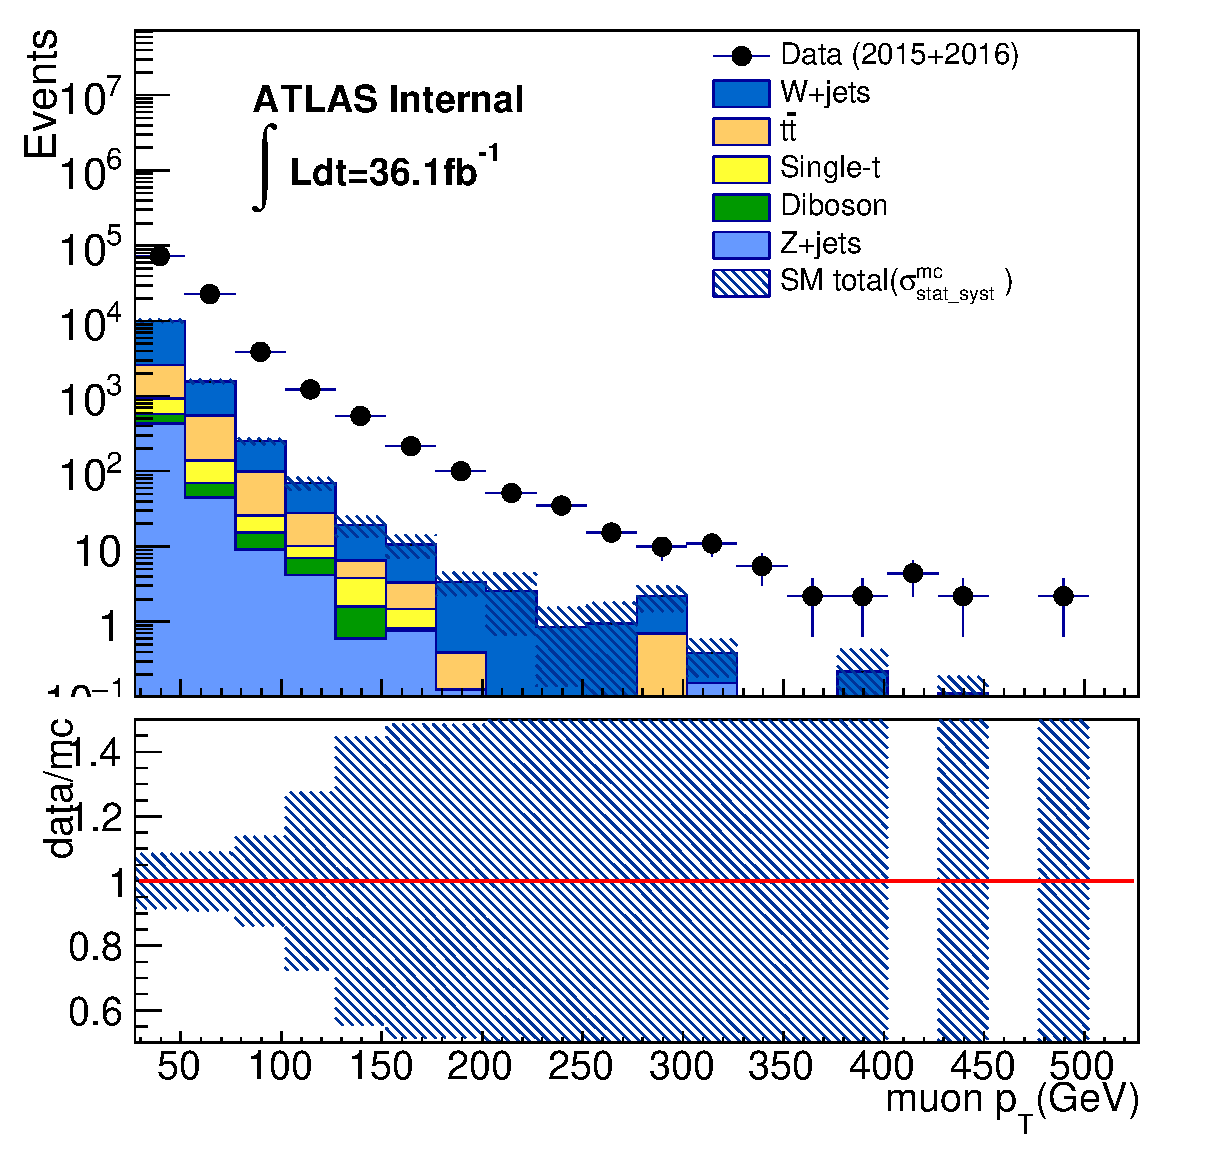
\includegraphics[width=0.45\textwidth]{Chapter3/MJ_CR/muonPt.eps}}
       \subfloat[]{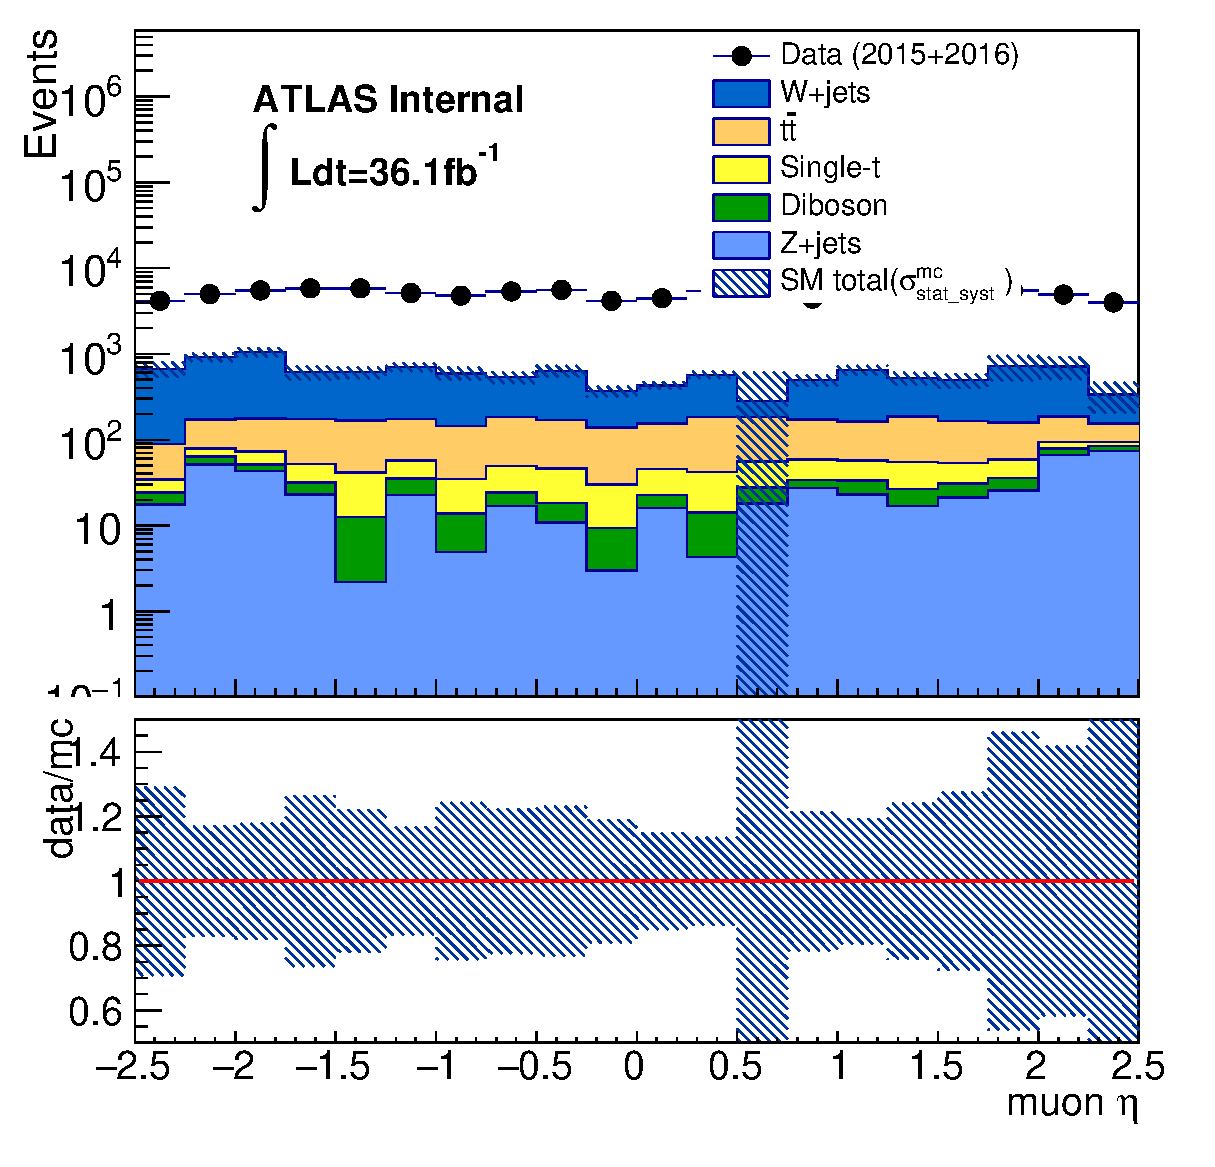
\includegraphics[width=0.45\textwidth]{Chapter3/MJ_CR/muonEta.eps}} \\
       \subfloat[]{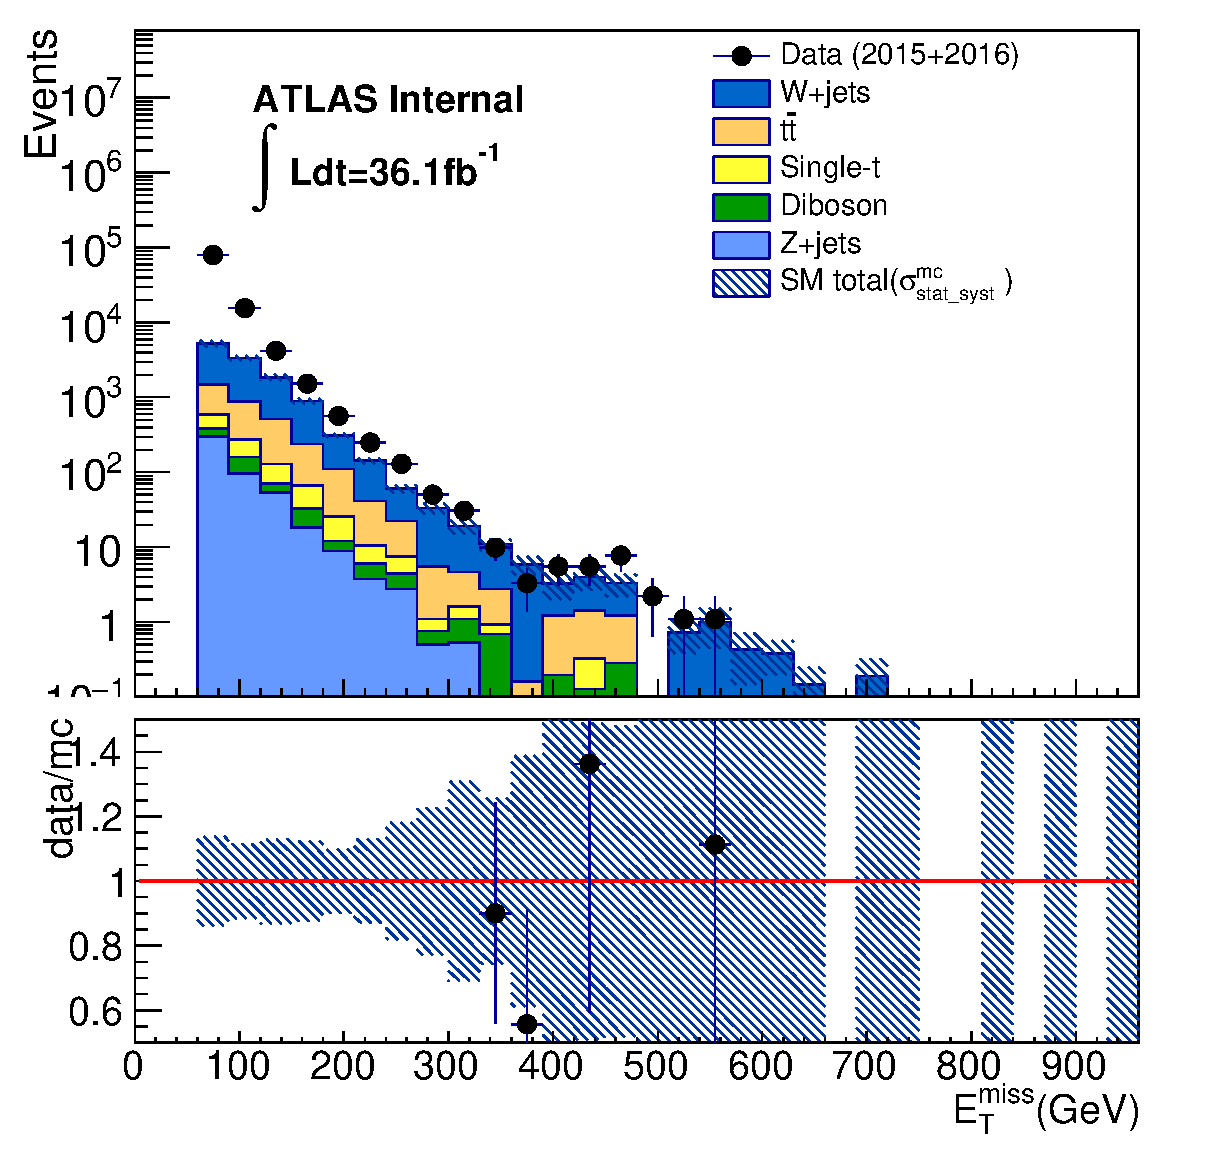
\includegraphics[width=0.45\textwidth]{Chapter3/MJ_CR/met_mu.eps}}
       \subfloat[]{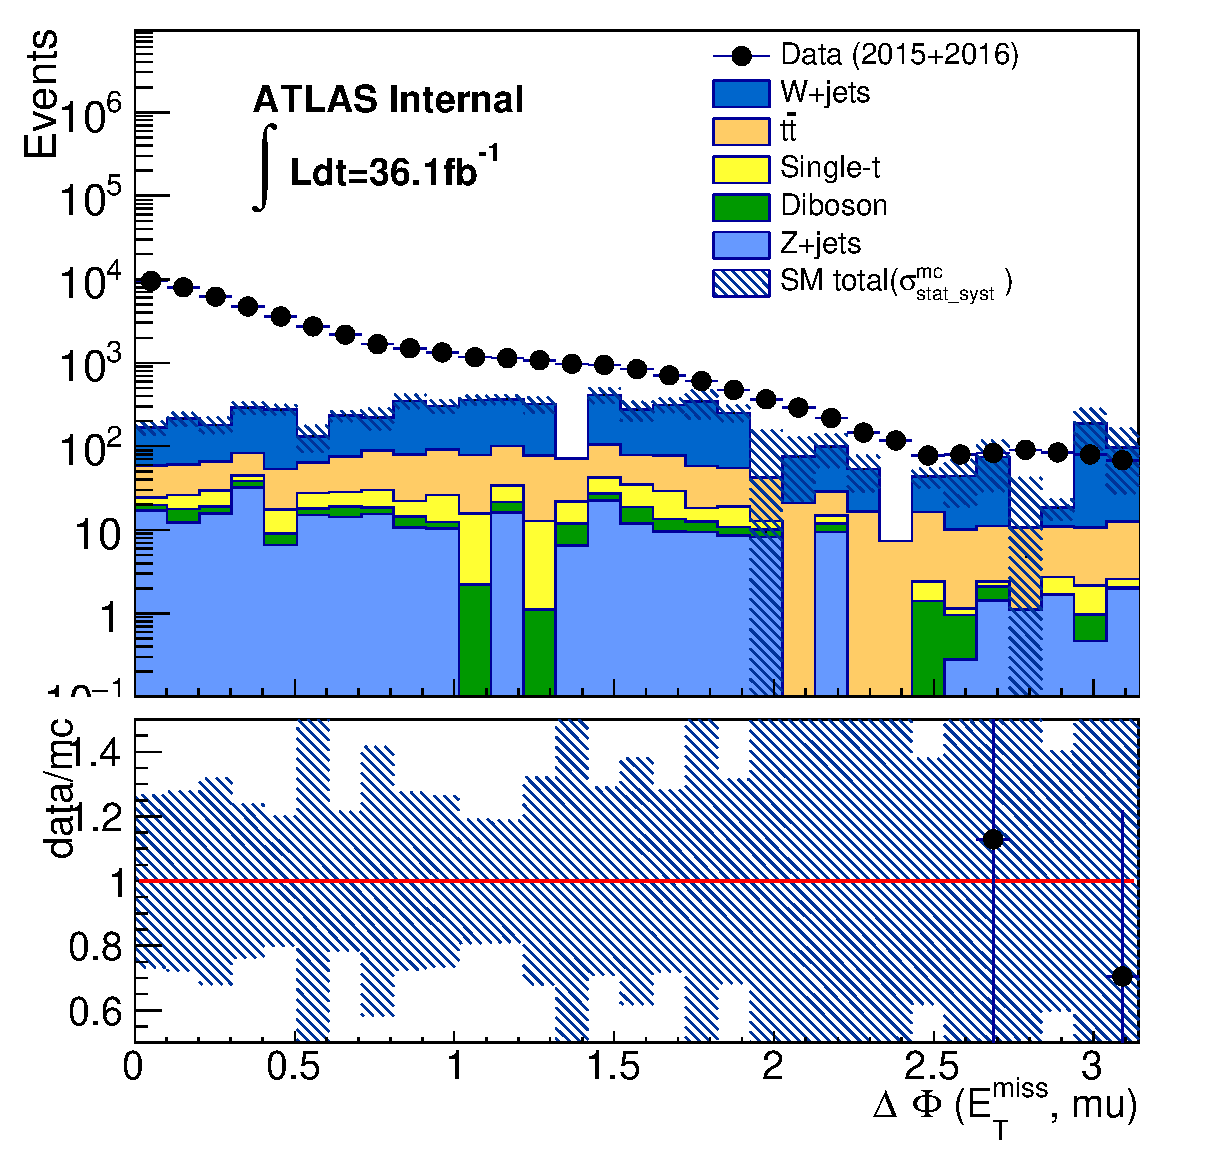
\includegraphics[width=0.45\textwidth]{Chapter3/MJ_CR/dphilepmet_mu.eps}}\\
       \caption{The distribution of lepton $p_{T}$,$\eta$, $E_{T}^{miss}$ and $\Delta\phi$($\mu$,$E_{T}^{miss}$) in dijet fake control region with inversed lepton for muon channel. The inconsistency is thought to be comprised of multijet events without applying electroweak subtraction.}
       \label{fig:dijetFakeCR_mu}
\end{figure}

\begin{table}[h]
  \caption{Electroweak subtraction factor for electron and muon channels} \label{tab:ewsubtraction}
  \begin{center}

    \begin{tabular}{ | c | c | c | }
     \hline
     channels                       &   electron   & muon \\ \hline
     EW subtraction factor          &   1.36       & 1.49 \\ \hline
\end{tabular}
\end{center}
\end{table}

\subsubsection*{Validation}
The method is validated in the dedicated validation region. The definition is similar to the signal region with looser cut to enrich the multijet events. It requires at lease two resolved jets ($p_{T}^{leading}>60GeV$, $p_{T}^{subleading}>45GeV$), $30GeV<E^{miss}_{T}<50GeV$, exactly one isolated lepton and the resolved triggers passed for electron and muon channels respectively. This definition is slightly overlapped with signal and control regions, but the upper cut on $E^{miss}_{T}$ suppress the signal contribution.  As the fake factors were derived from two bins of $p_{T}(l\nu)$, the validation is performed on $p_{T}(l\nu)<150 GeV$ and $p_{T}(l\nu)>150 GeV$. The results are presented in Figures~\ref{fig:FakeVR1_el} -~\ref{fig:FakeVR2_mu} with multijet background estimated using fake factor method. In general, data agrees well with backgrounds with tolerable inconsistency within statistic uncertainties. The disagreement in the region of $p_{T}(l\nu)>150 GeV$ is supposed to be due to the low statistics for fake factor estimation in single jet control region, but it should not have great impact in final interpretation, as multijet events would just account for around 10\% of the whole background. The related systematic uncertainty would be discussed in Chapter~\ref{Ch:resonance_stat}.
\clearpage
\begin{figure}[ht]
	\centering
	\subfloat[]{\includegraphics[width=0.43\textwidth]{Chapter3/MJ_VR/lep1pt_Loose_el_highWpt}}
	\subfloat[]{\includegraphics[width=0.43\textwidth]{Chapter3/MJ_VR/lep1eta_Loose_el_highWpt}}\\
	\subfloat[]{\includegraphics[width=0.43\textwidth]{Chapter3/MJ_VR/met_Loose_el_highWpt}}
	\subfloat[]{\includegraphics[width=0.43\textwidth]{Chapter3/MJ_VR/dphilepmet_Loose_el_highWpt}}\\
	\subfloat[]{\includegraphics[width=0.43\textwidth]{Chapter3/MJ_VR/lvjjmass_Loose_el_highWpt}}
	\caption{The distribution of lepton $p_{T}$,$\eta$, $E_{T}^{miss}$, $\Delta\phi$(e,$E_{T}^{miss}$), $m_{WV}$in validation region with $p_{T}(l\nu)>150 GeV$ in electron channel with multijet background}
	\label{fig:FakeVR1_el}
	
\end{figure}
\clearpage
\begin{figure}[ht]
	\centering
	\subfloat[]{\includegraphics[width=0.43\textwidth]{Chapter3/MJ_VR/lep1pt_Loose_el_lowWpt}}
	\subfloat[]{\includegraphics[width=0.43\textwidth]{Chapter3/MJ_VR/lep1eta_Loose_el_lowWpt}}\\
	\subfloat[]{\includegraphics[width=0.43\textwidth]{Chapter3/MJ_VR/met_Loose_el_lowWpt}}
	\subfloat[]{\includegraphics[width=0.43\textwidth]{Chapter3/MJ_VR/dphilepmet_Loose_el_lowWpt}}\\
	\subfloat[]{\includegraphics[width=0.43\textwidth]{Chapter3/MJ_VR/lvjjmass_Loose_el_lowWpt}}
	\caption{The distribution of lepton $p_{T}$,$\eta$, $E_{T}^{miss}$, $\Delta\phi$(e,$E_{T}^{miss}$), $m_{WV}$ and BDT in validation region with $p_{T}(l\nu)<150 GeV$ in electron channel with multijet background}
	\label{fig:FakeVR2_el}
\end{figure}
\clearpage
\begin{figure}[ht]
	\centering
	\subfloat[]{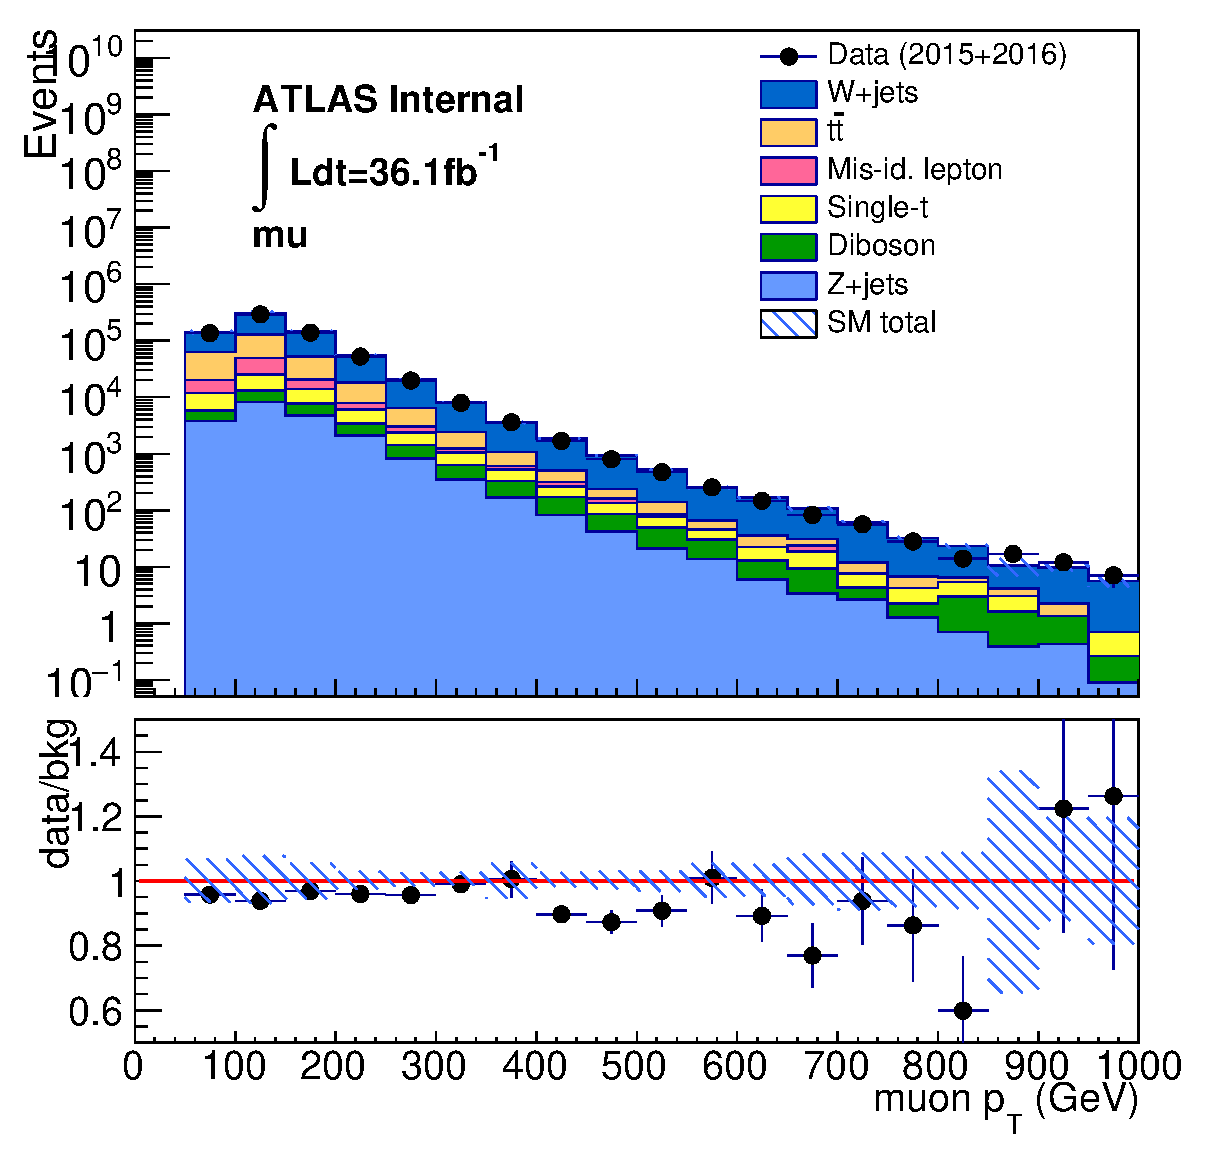
\includegraphics[width=0.43\textwidth]{Chapter3/MJ_VR/lep1pt_Loose_mu_highWpt.eps}}
	\subfloat[]{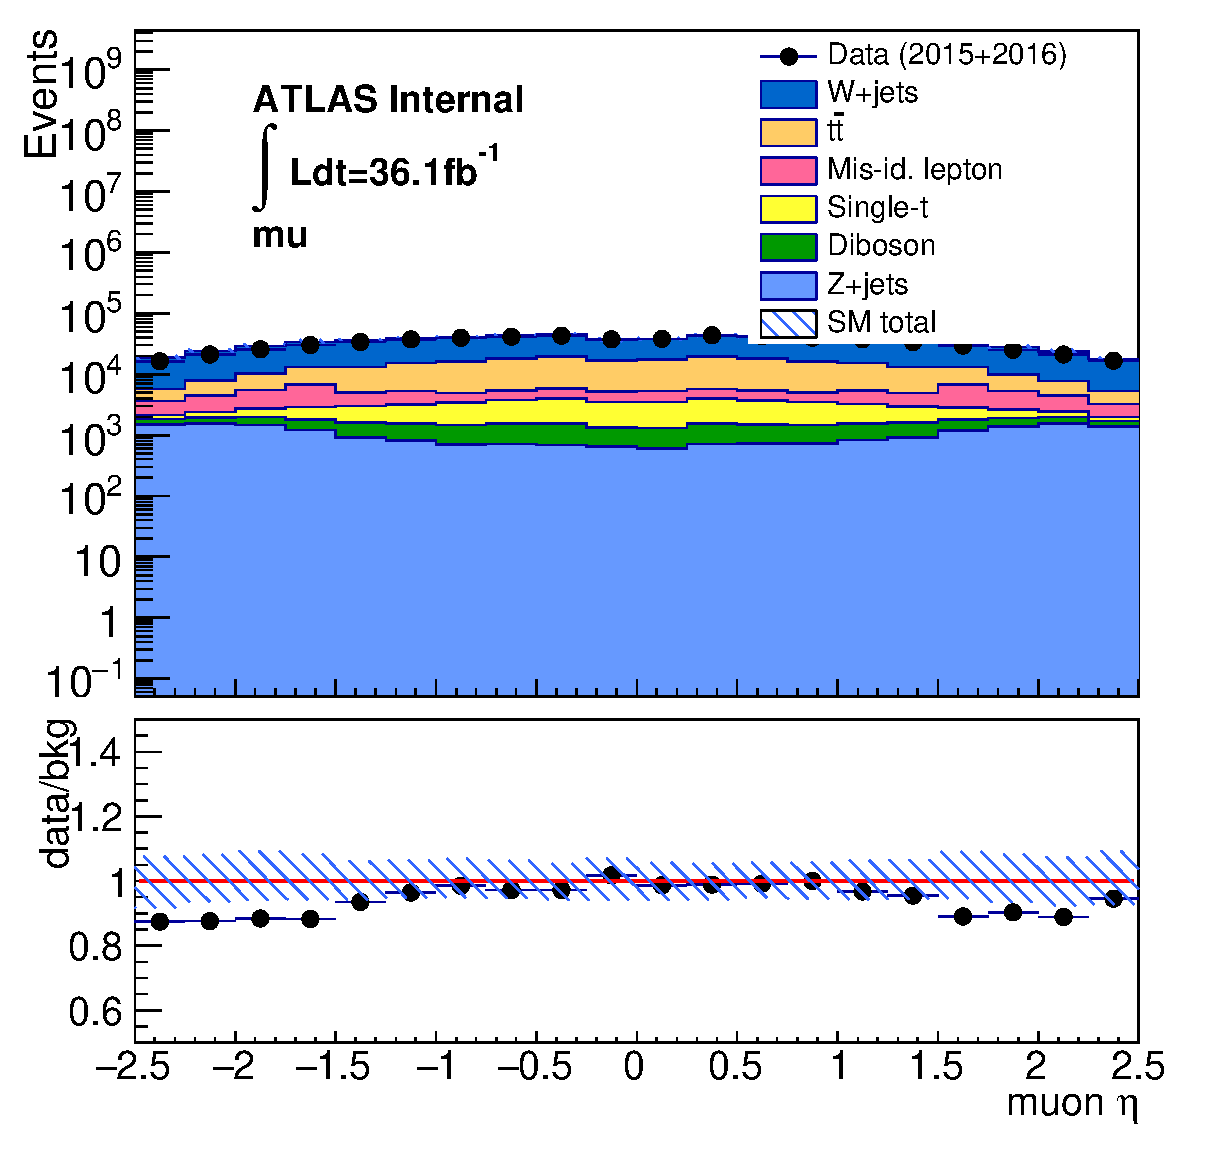
\includegraphics[width=0.43\textwidth]{Chapter3/MJ_VR/lep1eta_Loose_mu_highWpt.eps}}\\
	\subfloat[]{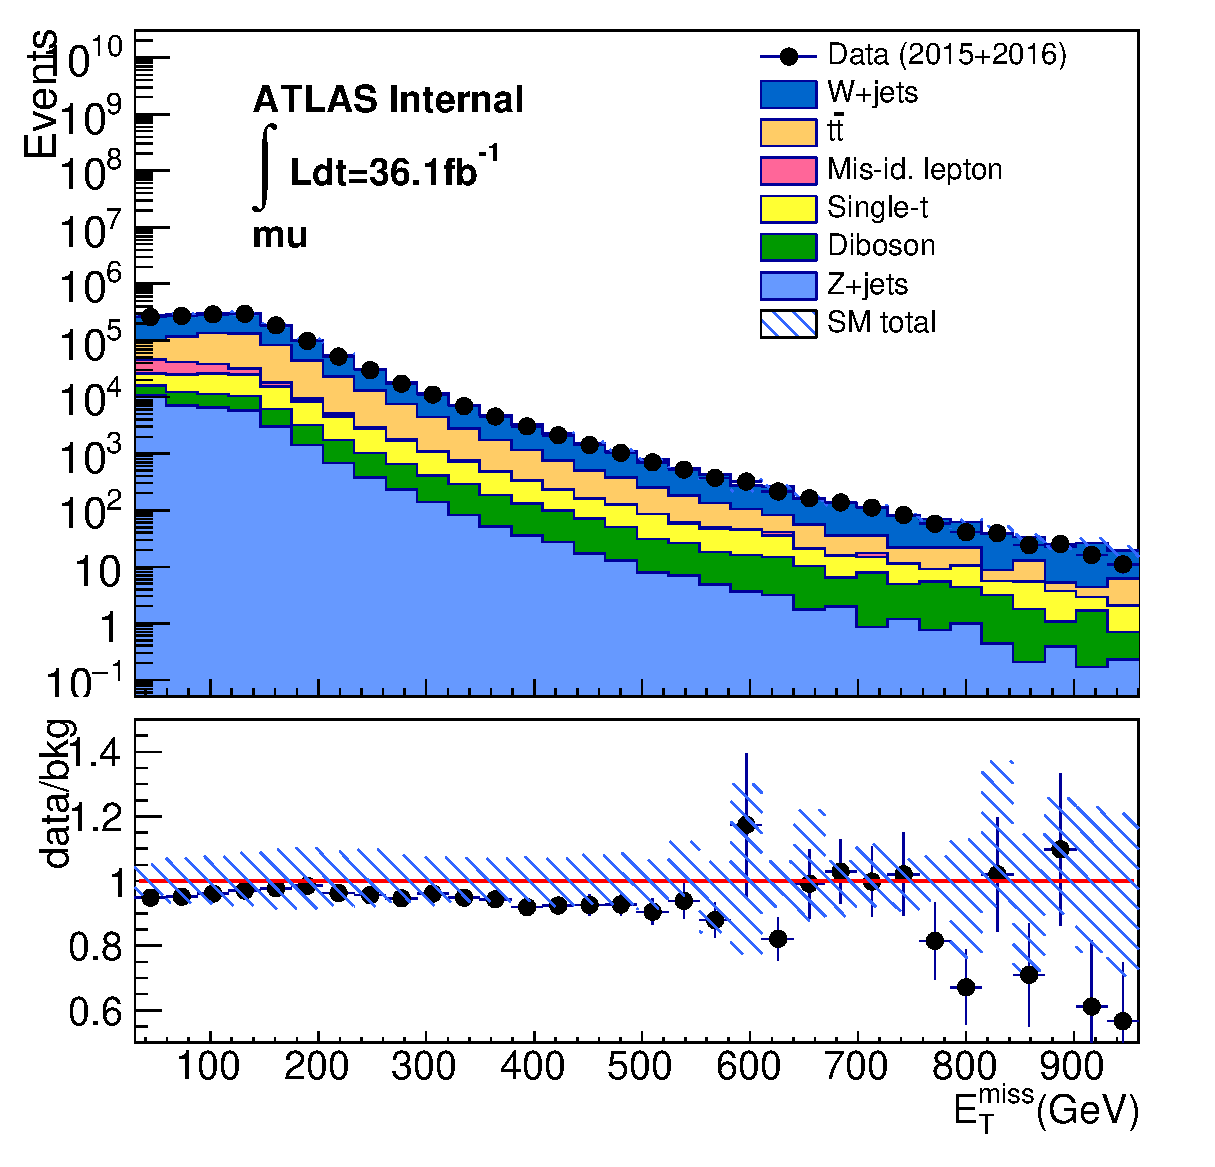
\includegraphics[width=0.43\textwidth]{Chapter3/MJ_VR/met_Loose_mu_highWpt.eps}}
	\subfloat[]{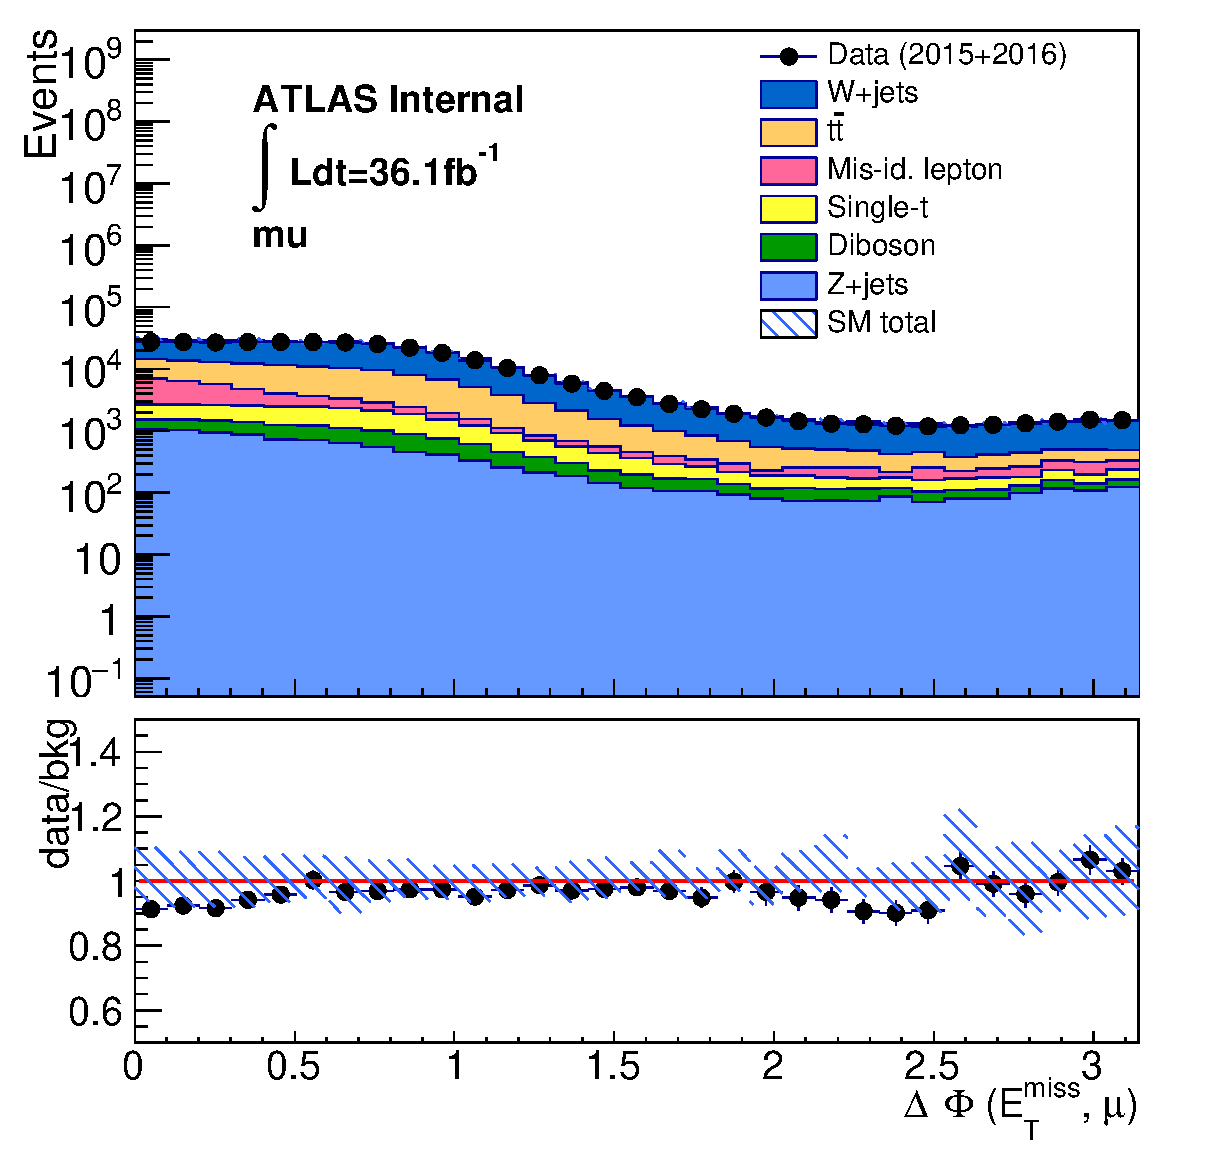
\includegraphics[width=0.43\textwidth]{Chapter3/MJ_VR/dphilepmet_Loose_mu_highWpt.eps}}\\
	\subfloat[]{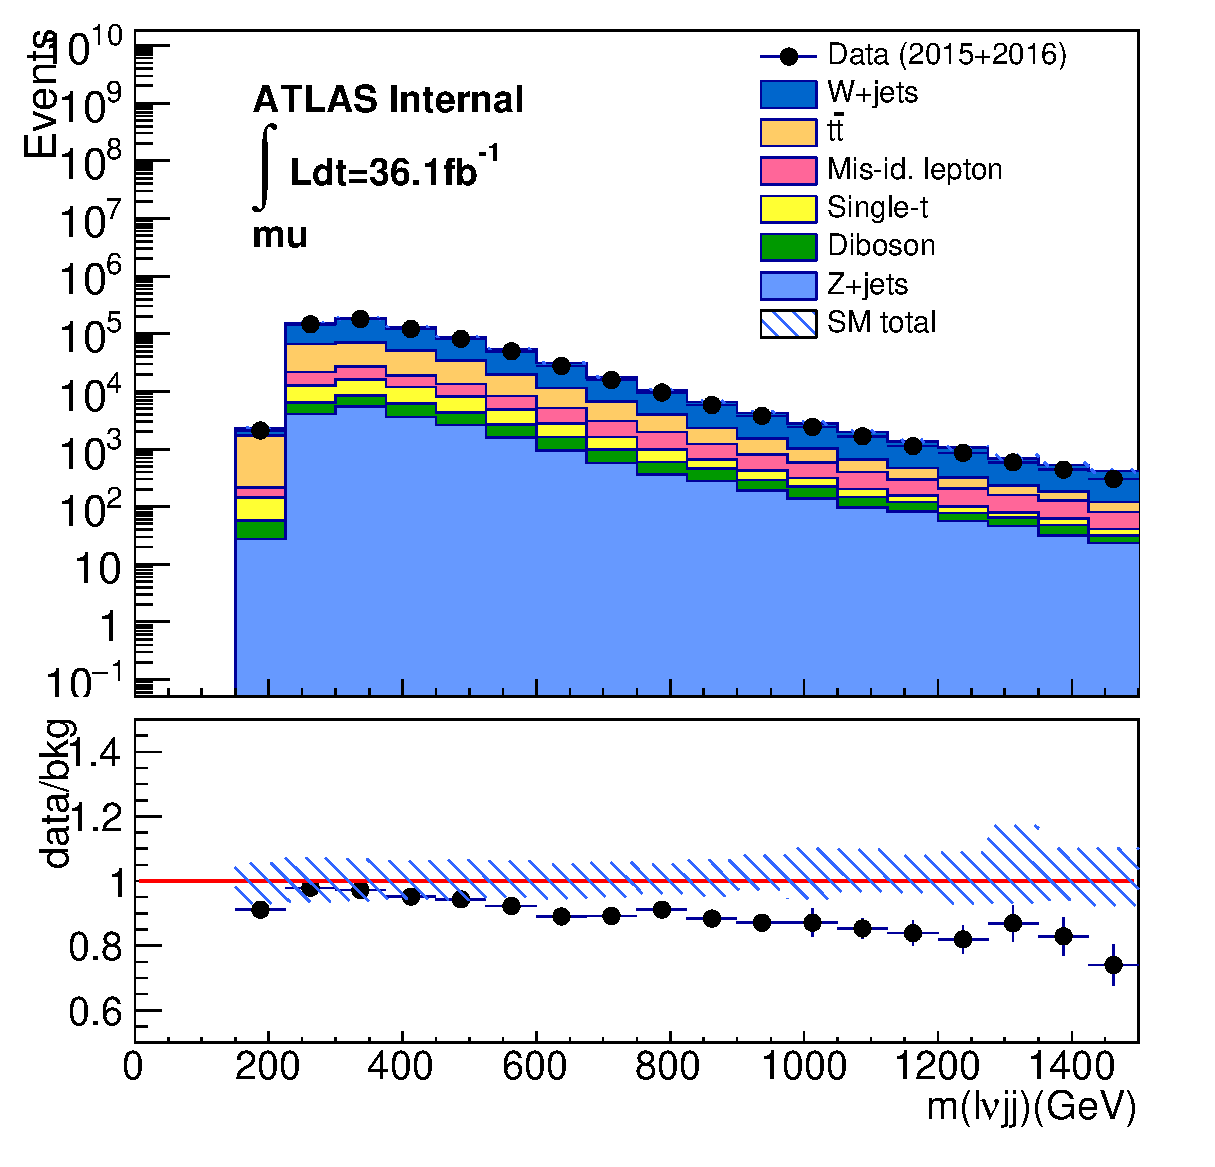
\includegraphics[width=0.43\textwidth]{Chapter3/MJ_VR/lvjjmass_Loose_mu_highWpt.eps}}
	\caption{The distribution of lepton $p_{T}$,$\eta$, $E_{T}^{miss}$, $\Delta\phi$($\mu$,$E_{T}^{miss}$), $m_{WV}$ and BDT in validation region with $p_{T}(l\nu)>150 GeV$ in muon channel with multijet background}
	\label{fig:FakeVR1_mu}
\end{figure}
\clearpage
\begin{figure}[ht]
	\centering
	\subfloat[]{\includegraphics[width=0.43\textwidth]{Chapter3/MJ_VR/lep1pt_Loose_mu_lowWpt.eps}}
	\subfloat[]{\includegraphics[width=0.43\textwidth]{Chapter3/MJ_VR/lep1eta_Loose_mu_lowWpt.eps}}\\
	\subfloat[]{\includegraphics[width=0.43\textwidth]{Chapter3/MJ_VR/met_Loose_mu_lowWpt.eps}}
	\subfloat[]{\includegraphics[width=0.43\textwidth]{Chapter3/MJ_VR/dphilepmet_Loose_mu_lowWpt.eps}}\\
	\subfloat[]{\includegraphics[width=0.43\textwidth]{Chapter3/MJ_VR/lvjjmass_Loose_mu_lowWpt.eps}}
	\caption{The distribution of lepton $p_{T}$,$\eta$, $E_{T}^{miss}$, $\Delta\phi$($\mu$,$E_{T}^{miss}$), $m_{WV}$ and BDT in validation region with $p_{T}(l\nu)<150 GeV$ in muon channel with multijet background}
	\label{fig:FakeVR2_mu}
\end{figure}
\clearpage
\section{Data Background Comparison}
\label{Sec:data_bkg_compar}
To verify the modelling of background estimation, the comparison in top and W+jet control regions are performed for both VBF and ggF categories. The consistency is not perfect as expectation, and the fitting in the control regions is on the purpose to recover it, which will be discussed in next chapter. The other issue in the background simulation is that a slope in the ratio of data over background is observed in $m^{VBF}_{jj}$ in resolved VBF category for V+jet samples from Sherpa generator. In this analysis, it is also taken as one contribution to the mismodelling of simulation. 
\\
\\Fig. \ref{Fig:ggFWR} and Fig. \ref{Fig:ggFTR} are the comparison plots for $m_{WV}$ in ggF category, while Fig. \ref{Fig:mWVVBFWR} to Fig. \ref{Fig:mWVVBFTR} are for VBF category. The comparison of  $m^{VBF}(j,j)$ could be found in Fig. \ref{Fig:mJJVBFWR} and Fig. \ref{Fig:mJJVBFTR} to examine the VBF modelling. 
\newpage

\begin{figure}[ht]
	\centering
	\subfloat[]{\includegraphics[width=0.43\textwidth]{Chapter3/HighPurityCR_36fb/VVM_3_el}}
	\subfloat[]{\includegraphics[width=0.43\textwidth]{Chapter3/HighPurityCR_36fb/VVM_3_mu}}\\
	\subfloat[]{\includegraphics[width=0.43\textwidth]{Chapter3/LowPurityCR_36fb/VVM_12_el}}
	\subfloat[]{\includegraphics[width=0.43\textwidth]{Chapter3/LowPurityCR_36fb/VVM_12_mu}}\\
    \subfloat[]{\includegraphics[width=0.43\textwidth]{Chapter3/ResolvedCR/ggF36fb/VVM_5_el}}
	\subfloat[]{\includegraphics[width=0.43\textwidth]{Chapter3/ResolvedCR/ggF36fb/VVM_5_mu.eps}}
	\caption{The distribution of $m_{WV}$ in ggF high purity (top), low purity (middle), and resolved (bottom) W+jet control region for electron (left) and muon (right) channels respectively}
	\label{Fig:ggFWR}
\end{figure}



\begin{figure}[ht]
	\centering
	\subfloat[]{\includegraphics[width=0.43\textwidth]{Chapter3/HighPurityCR_36fb/VVM_2_el}}
	\subfloat[]{\includegraphics[width=0.43\textwidth]{Chapter3/HighPurityCR_36fb/VVM_2_mu}}\\
	\subfloat[]{\includegraphics[width=0.43\textwidth]{Chapter3/LowPurityCR_36fb/VVM_13_el}}
    \subfloat[]{\includegraphics[width=0.43\textwidth]{Chapter3/LowPurityCR_36fb/VVM_13_mu}}\\
	\subfloat[]{\includegraphics[width=0.43\textwidth]{Chapter3/ResolvedCR/ggF36fb/VVM_6_el}}
    \subfloat[]{\includegraphics[width=0.43\textwidth]{Chapter3/ResolvedCR/ggF36fb/VVM_6_mu.eps}}
	\caption{The distribution of $m_{WV}$ in ggF high purity (top), low purity (middle), and resolved (bottom) top control region for electron (left) and muon (right) channels respectively}
	 \label{Fig:ggFTR}
\end{figure}


\begin{figure}[ht]
	\centering
	\subfloat[]{\includegraphics[width=0.43\textwidth]{Chapter3/VBF36fbHP/VVM_3_el}}
	\subfloat[]{\includegraphics[width=0.43\textwidth]{Chapter3/VBF36fbHP/VVM_3_mu}}\\
	\subfloat[]{\includegraphics[width=0.43\textwidth]{Chapter3/VBF36fbLP/VVM_12_el}}
    \subfloat[]{\includegraphics[width=0.43\textwidth]{Chapter3/VBF36fbLP/VVM_12_mu}}\\	
	\subfloat[]{\includegraphics[width=0.43\textwidth]{Chapter3/ResolvedCR/VBF36fb/VVM_5_el}}
    \subfloat[]{\includegraphics[width=0.43\textwidth]{Chapter3/ResolvedCR/VBF36fb/VVM_5_mu.eps}}    
	\caption{The distribution of $m_{WV}$ in VBF high purity (top), low purity (middle), and resolved (bottom) W+jet control region for electron (left) and muon (right) channels respectively}
	\label{Fig:mWVVBFWR}
\end{figure}
\clearpage
\begin{figure}[ht]
	\centering

	\subfloat[]{\includegraphics[width=0.43\textwidth]{Chapter3/VBF36fbHP/VBFmass_3_el}}
	\subfloat[]{\includegraphics[width=0.43\textwidth]{Chapter3/VBF36fbHP/VBFmass_3_mu}}\\
	\subfloat[]{\includegraphics[width=0.43\textwidth]{Chapter3/VBF36fbLP/VBFmass_12_el}}
    \subfloat[]{\includegraphics[width=0.43\textwidth]{Chapter3/VBF36fbLP/VBFmass_12_mu}}\\	
 	\subfloat[]{\includegraphics[width=0.43\textwidth]{Chapter3/ResolvedCR/VBF36fb/VBFmass_5_el}}
    \subfloat[]{\includegraphics[width=0.43\textwidth]{Chapter3/ResolvedCR/VBF36fb/VBFmass_5_mu}}\\   
	\caption{The distribution of $m_{jj}^{VBF}$ in VBF high purity (top), low purity (middle), and resolved (bottom) W+jet control region for electron (left) and muon (right) channels respectively}
	\label{Fig:mJJVBFWR}
\end{figure}


\begin{figure}[ht]
	\centering
	\subfloat[]{\includegraphics[width=0.43\textwidth]{Chapter3/VBF36fbHP/VVM_2_el}}
	\subfloat[]{\includegraphics[width=0.43\textwidth]{Chapter3/VBF36fbHP/VVM_2_mu}}\\
	\subfloat[]{\includegraphics[width=0.43\textwidth]{Chapter3/VBF36fbLP/VVM_13_el}}
    \subfloat[]{\includegraphics[width=0.43\textwidth]{Chapter3/VBF36fbLP/VVM_13_mu}}\\
	\subfloat[]{\includegraphics[width=0.43\textwidth]{Chapter3/ResolvedCR/VBF36fb/VVM_6_el}}
    \subfloat[]{\includegraphics[width=0.43\textwidth]{Chapter3/ResolvedCR/VBF36fb/VVM_6_mu.eps}}	
	\caption{The distribution of $m_{WV}$ in VBF high purity (top), low purity (middle), and resolved (bottom) top control region for electron (left) and muon (right) channels respectively}
	\label{Fig:mWVVBFTR}
\end{figure}
\clearpage
\begin{figure}[ht]
	\centering
	\subfloat[]{\includegraphics[width=0.43\textwidth]{Chapter3/VBF36fbHP/VBFmass_2_el}}
	\subfloat[]{\includegraphics[width=0.43\textwidth]{Chapter3/VBF36fbHP/VBFmass_2_mu}}\\
	\subfloat[]{\includegraphics[width=0.43\textwidth]{Chapter3/VBF36fbLP/VBFmass_13_el}}
    \subfloat[]{\includegraphics[width=0.43\textwidth]{Chapter3/VBF36fbLP/VBFmass_13_mu}}\\	
    \subfloat[]{\includegraphics[width=0.43\textwidth]{Chapter3/ResolvedCR/VBF36fb/VBFmass_6_el}}
    \subfloat[]{\includegraphics[width=0.43\textwidth]{Chapter3/ResolvedCR/VBF36fb/VBFmass_6_mu}}\\
	\caption{The distribution of $m_{jj}^{VBF}$ in VBF high purity (top), low purity (middle), and resolved (bottom) top control region for electron (left) and muon (right) channels respectivelyy}
	\label{Fig:mJJVBFTR}
\end{figure}

